%%%       aums.sty (Masters Thesis)
%%%       auphd.sty (Ph.D. Dissertation)
%%%       auhonors.sty (Honors Scholar)

%%%To use it, please edit the necessary options, title, author, date, year, keywords, advisor, professor, etc. 

\documentclass[12pt]{report}
%\usepackage{aums}       % For Master's papers
\usepackage{auphd}     % Rodney edited the aums style to auphd
\usepackage{ulem}       % underlining on style-page; see \normalem below
\usepackage{url}
\usepackage{tikz}
\usepackage{pgf}
\usepackage{graphicx}
\graphicspath{ {./images} }
\usepackage{todonotes}
\usepackage{mathtext}
\usepackage{listings}
\usepackage{pgfgantt}
\usepackage{comment}
\usepackage{adjustbox}
\usepackage{outlines}
%\usepackage[table]{xcolor}
\usepackage{algorithm} 
\usepackage{algpseudocode}
%\usepackage{natbib}
%%%%%Format rules: Normal margins are 1 in. If you need to print with 1.5in margins, uncomment the line below
%\oddsidemargin0.5in \textwidth6in

%% If you do not need a List of Abbreviations, then comment out the lines below and the \printnomenclature line.
%%for List of Abbreviations information:  (see http://www.mackichan.com/TECHTALK/509.htm  )
\usepackage[intoc]{nomencl}
\renewcommand{\nomname}{List of Abbreviations}   	       
\makenomenclature 
%% don't forget to run:   makeindex ausample.nlo -s nomencl.ist -o ausample.nls
%% Also, if 

% May want theorems numbered by chapter
\newtheorem{theorem}{Theorem}[chapter]

% Put the title, author, and date in. 
\title{Software Forensics for Adversarial Authorship}
\author{Rodney Visser} 
\date{[Insert date of graduation, e.g., Aug 1, 2023]} %date of graduation
\copyrightyear{2023} %copyright year

\keywords{Software Forensics, Threat TTPs, Digital Provenance, Machine Learning, Deep Neural Networks, Random Forrest Classifier, Threat Intelligence, Authorship Attribution}

% Put the Thesis Adviser here. 
\adviser{David Umphress}

% Put the committee here (including the adviser), one \professor for each. 
% The advisor must be first, and the dean of the graduate school must be last.
% WHY IS THIS NOT SHOWING UP ON THE TITLE PAGE???
\professor{David Umphress, Chair, Emeritus Professor of Computer Science and Software Engineering}
\professor{Daniel Tauritz, Associate Professor of Computer Science and Software Engineering}
\professor{Anthony Skjellum, Professor and SimCenter Director, University of Tennessee Chattanooga}
\professor{Drew Springall, Assistant Professor of Computer Science and Software Engineering}

\begin{document}
\begin{romanpages}      % roman-numbered pages 
\TitlePage 

\begin{abstract} 
Software forensics in computer science can often be used to determine intellectual property rights and it provides potential for threat attribution.  Risks from malicious software and the software supply chain are becoming increasingly an issue as code gets more complex and attackers continuously outpace defenders in the digital domain.  The software development process has changed significantly and threats have been on the bleeding edge of this maturity in terms of capability and obfuscation. The history and modern motivation for such analysis of software is present and includes commercial and government organizations.  This research investigates current static and dynamic methods of performing software forensics and improves on these methods by utilizing multi-dimensional analysis to detect semantic differences between two versions of a similar software code and then applying models in order to predict future changes in behavior.
\end{abstract}

%\begin{acknowledgments}
%Put text of the acknowledgments here.
%\end{acknowledgments}

\tableofcontents
\listoffigures
%\listoftables

\printnomenclature[0.5in] %used for the List of Abbreviations
\end{romanpages}        % All done with roman-numbered pages


\normalem       % Make italics the default for \em
%*********************************************************************
%*********************************************************************
%Chapter One (CH1)
%*********************************************************************
%*********************************************************************
\chapter{Introduction}  
\label{chap:one}

A quickly growing use case of software forensics is authorship attribution, the process of attempting to identify the likely authorship of a software sample given a collection of software whose authorship is known.  Convention points to the use of a subfield of digital forensics, software forensics,  to apply authorial context to the providence of malicious software.  The categorization and mapping of key properties extracted from a suspect artifact can be used to select candidate matches from a pool of legitimate artifacts.

Currently, reverse engineering software artifacts suspected of being malicious code remains a labor-intensive and manual task, despite advances in automated programming understanding.  Static and dynamic analysis tools provide insight into software structure and behavior, but the ultimate determination of what is a malicious artifact relies heavily on the skills and experiences of individual forensic investigators.  Further complicating the process, attackers have also begun to place false flags within the technical breadcrumbs that are commonly left behind after a cyber attack.  The means of which threats deliver malicious code has changed along with complexity of false flags.  Typically modern threats interface with how users interact with the internet and network around them. 

A cost effective example of malware delivery is through the use of phishing emails, where the content of the email tries to entice the recipient to click a URL linking to a malicious web site or downloading a malicious attachment. Analysts attempting to provide intelligence on such activities quickly find that the ever increasing volume of phishing emails circulating daily is overwhelming and the most effective phishing techniques are often not caught because of their use of the proper application of backstopping.  Therefore, intelligence gathered within this area is only representative of only a small sample at a single point in time, not of the global picture of the problem.  Additionally, analyses have revealed that authorship attribution on this type of malware delivery method have provided linkages to the same author, but that it is unlikely that the authorship-based clustering algorithms have managed to group together all spam produced by each group.  Said in another way, this is not a sustainable answer to authorship attribution on this type of malware delivery method on it's own because of the low rate of recall within APT groups.  This problem of high precision with low recall has been faced in past authorship research \cite{li2017association}.  In broader terms, the issue of authorship attribution of malicious code and the various delivery methods suffer from problems related to precision and recall when analyzed on their own.  This problem we propose can be assisted by multi-dimensional analysis using a novel framework.

A key issue in authorship attribution for cyber attacks is the lack of specific knowledge about technical capabilities, motivation, policies, and laws that currently govern this area.  The difficult technical side of attribution is further escalated by serious legal and policy questions about when and how to accuse governments of responsibility for cyber attacks.  Within the area of technical capabilities and motivations for groups that have been labeled as Advanced Persistent Threats (APT)s by commercial cyber security firms, there are sweeping differences in the arrangement, categorization, and number of named threats from nation states or criminal enterprises \cite{romanosky2019private}.  Below in Table 1.1 we provide a snapshot of the disconnect between leading cyber threat intelligence firms that track and publish intelligence on named APTs.

\begin{table}[h!]
  \centering
    \caption{Named APTs}
    \label{tab:table1}
    \begin{adjustbox}{width=\textwidth}
    \begin{tabular}{l|c|c|c|c|c} % <-- Alignments: 1st column left, 2nd middle and 3rd right, with vertical lines in between
      \textbf{Country} & \textbf{FireEye} & \textbf{CrowdStrike}  & \textbf{Kaspersky} & \textbf{Dell SecureWorks}  & \textbf{Cisco Talos}\\
      \hline
      China & 20 & 40 & N/A & 5 & 9 \\
      Russia & 3 & 3 & N/A & 6 & 3 \\
      Iran & 3 & 7 & N/A & 1 & 3 \\
      North Korea & 1 & 4 & N/A & 2 & 2 \\
      Criminal / Terrorist & 10 & 29 & N/A & 3 & 1 \\
      Other & 2 & 1 & N/A & 2 & - \\ 
      Unknown/Undisclosed & 8 & 1 & N/A & - & 1 \\
      \hline
      Total & 47 & 85 & 36 & 19 & 19\\
    \end{tabular}
  \end{center}
\end{table}

Although politics may largely determine whether attributions are made public, there is a need for a framework in which cyber attacks are attributed to states in a means governed by legal standards \cite{eichensehr2020law}.  Experts on the topic of cyber threat attribution are quick to call for greater levels of regulation and policy that govern the world's critical infrastructure and economies, but for the most part, worldwide leaders in key positions do not understand the issues presented to them, the proper information is not made available, or the terrain of navigating the geopolitical landscape on this issue in the public eye is deemed risky.

A prime example of state-sponsored cyber espionage and influence operations is the unauthorized access and disclosure of the Democratic party's email in 2016 by a Russian State backed hacker group commonly referred to as Fancy Bear.  The main point of dissemination for this operation was a self proclaimed Romanian hacker called Guccifer 2.0.  Toni Gidwani, director of research operations for ThreatConnect, said: ``It would suggest to us that the operators of the Guccifer 2.0 persona were not the actors who breached the DNC.  You’re looking at the operations guys who don’t have the same technical credibility as these very sophisticated actors who exploited these networks. You've got a lot of cooks in this kitchen here, not just one actor.'' \cite{zager2016response}

This type of misdirection campaign for state-sponsored hacking is considered common place and automated single-dimension attribution techniques are easily guided in the wrong direction.  Recent application of technology in the realm of source code authorship attribution methods have accuracy above 88\%, but adversarial learning attack methods drop the rates of attribution to around 1\% \cite{abuhamad2018large}, \cite{caliskan2015anonymizing}, \cite{quiring2019misleading}. 

For these reasons, attribution must be thought of as a multi-dimensional issue that draws on multiple sources of information available, including technical forensics, human intelligence, signals intelligence, history, and geopolitics, among others \cite{lin2016attribution}.  If successful, the attribution of successful adversarial attacks from code left behind on an infected system could enable software forensics to be leveraged in order to be fight advancing and evolving threats. 

\begin{comment}
Why it is important 
    - expert opinions - if only we could apply attribution
	    2016 presidential election
	    Olymipics hack (Wired)
	    Sony hack

    - number statistics
        attack has a substantial effect on two recent attribution methods,  whose accuracy drops from over 88 percent to 1 percent under attack.
    
        [1] M. Abuhamad, T. AbuHmed, A. Mohaisen, and D. Nyang. Large-scale and language-oblivious code authorship identification. In Proc. of ACM Conference on Computer and Communications Security (CCS), 2018.
@inproceedings{abuhamad2018large}

        [9] A. Caliskan, R. Harang, A. Liu, A. Narayanan, C. R. Voss, F. Yamaguchi, and R. Greenstadt. Deanonymizing programmers via code stylometry. In Proc. of USENIX Security Symposium, 2015.
@inproceedings{caliskan2015anonymizing}

	DU "I don't get a scense of the degree to which the problem is relevant.  Please provide information which points to the impoertance of solving the problem.  Substantiate with facts."

A. INSERT Ref to "ODNI_A_Guide_to_Cyber_Attribution"
"Establishing attribution for cyber operations is difficult but not impossible.  No simple technical process or automated solution for determining responsibility for cyber operations exists.  The painstaking work in many cases requires weeks or months of analyzing intelligence and forensics to assess culpability.  In some instances, the IC can establish cyber attribution within hours of an incident but the accuracy and confidence of the attribution will vary depending on available data."


Addin Bruce Scnider reference on threat attribution and one from ex-Microsoft Executive that was the Cyber Czar and incorrect about China." Howard Anthony Schmidt died in 2017 at the age of 67

E G See, Rt, Philip Hon, Hammond
I unequivocally condemn these cyber attacks [on Sony] and am deeply concerned at the findings of the US investigation, which seems to provide further evidence of North Korea's blatant disregard for international norms and obligations
Foreign & Commonwealth Off
Posted: 2014-12-19

E G See, Bruce Schneier
I am deeply skeptical of the FBI's announcement on Friday that North Korea was behind last month's Sony hack. The agency's evidence is tenuous, and I have a hard time believing it
Posted: 2014-12-22

E G See, Jack Goldsmith
sony-hack-attribution-problemsand-connection-domestic-surveillance (noting that "the 'evidence' is of the most conclusory nature" and "on its face . . . shows only that this attack has characteristics of prior attacks attributed to North Korea
Posted: 2014-12-19
\end{comment}

\section{Software Forensics}
\begin{comment}
The history of software forensics is a relatively brief one when compared to other forensic sciences.  It began with methods for finding similarities in software by comparing code through hashing, statistical analysis, text matching, and tokenization.  These methods compared software code at a primitive level by ingesting sources and producing a single measure indicating similarity.  These measures were not accurate enough to be admissible in modern courts because the algorithms used to find them could be easily fooled by simple substitutions.  ``The discipline of computer forensics appears to be struggling over methods and practices that will meet the courts’ “standards” for scientific evidence" \cite{meyers2005digital}.

By first examining similarity of a software artifact to other artifacts that have been previously observed, investigators can frame deeper questions, such as investigating new or changed capabilities.  For example, clues as seemingly insignificant as the format of calendar dates or the language used in text strings can be used to help identify demographic origins.  Level of sophistication, control flow patterns, stylistic flourishes, obfuscation techniques, and unique defects have the potential to signal the education and skill level of an artifacts creator or creators, perhaps going so far as to call out our artifact authorship given a collection of samples from a known author or authors.  Indirect information of this type, if available and used properly, offers a context so that investigators are not working in a vacuum, where each suspect artifact has been treated as a never-before-seen item.

The challenge becomes one of how to automate the use of attributes as figurative fingerprints capable of leading software forensic investigators to artifact lineage and pedigree.  Principal unresolved issues include how to identify which attributes determine similarity among artifacts, how to assess the trust of information inferred from the use of attributes, and how to establish a sufficiently reliable approach to satisfy legal standards.

\section{Problem Statement}
\label{sec:ProbState}
\end{comment}

Within the questions of what, when, where, who, and how for digital forensic investigations, answering the who question is frequently the most elusive.  The strategic aim of this research is to assist in answering this important question.  The tactical objectives include a survey of current state-of-the-art techniques in adversarial authorship using software forensics and the application of machine learning to automate and innovate analysis.

Software-assisted detection allows vast collections of artifacts to be compared to each other, making successful detection much more likely than traditional manual methods.  We refer to these first generation software-assisted means of detection as Single Dimensional Software Correlation.  This method can be thwarted by simple compiler optimizations and anti-forensic techniques.  Differences in hashing and mapping methods can cause a significant increase in false negatives count.

The motivation to use more focused and robust software forensic techniques is growing at an expanded rate in order to keep up with the adversarial techniques malware authors use to obfuscate their code.  Cyber threat actors for the most part are out pacing the defenders at an increasing rate, modern software forensics tools, techniques, and procedures are growing, but not fast enough to lessen the gap with threats.  In order to keep pace with intermediate and advanced level threat actors, novel techniques must be employed to find, track, and project how threats are evolving.  It is our belief that adversarial authorship using software forensics can allow us to do this.

%********************************************************************
%********************************************************************
%Chapter Two (CH2)
%********************************************************************
%********************************************************************
\chapter{Literature Survey}
\label{chap:two}
Using software forensics to track and plot the actions and potential growth of cyber threat actors includes problematic factors such as: lowered barriers of entry in terms of technical competence, malware as a service platforms, increasing levels of sophistication, and an rapidly expanding attack surface.  Authorship attribution has its roots in plagiarism detection, which is the process of locating instances of literary theft within traditional documents.  The modern day widespread use of computers connected to the Internet has eased the task of the plagiarist.  A great deal of cases of plagiarism can be found in academia, where documents are typically essays or reports, but plagiarism can be found in virtually any field, including software engineering. \cite{!stealsc:2012}  Research on plagiarism is described as an open problem, in that you can compare source documents to detect content plagiarized from such sources.  \cite{buruiana2013automatic}, \cite{jhivapd}

In the case of software plagiarism, advanced obfuscation techniques have made automated detection at scale increasingly difficult because of the ease of change in the structure of the code while preserving the code semantics \cite{xu2020revisiting}.  As an example, software compilers can easily configured to obfuscation techniques to change the assembly code, resulting in a low similarity score.  For prototypes that have been seen to be resilient to advanced code obfuscation, there is a problem of scale.  Most graph-based approaches are time consuming since it is a NP-hard problem.  Within an example of semantics-based approach using graphs, it took an hour in  the  comparison \emph{thttpd} and \emph{sthttpd}, and half a day in the comparison between \emph{Gecko} and \emph{Firefox} \cite{luo2014semantics}.  Given the increased application of advanced obfuscation techniques to malware, the scalability to process samples becomes a critical need.

The development of a novel graph pruning technique has shown that software correlation can be used to understand how malicious code has evolved over the years, and in particular, how different instances of malicious code relate to one another \cite{gupta2009empirical}.  Researchers established an inheritance relationships between different instances of malware based on temporal information and key common phrases identified in the malware descriptions and an extension of this research has the potential to show that software correlation can be used to inspect known examples of malware in order to gauge how threats and their code bases are successfully attributed and evolving.

Authorship attribution for malware has roots in traditional author identification in books, software intellectual property rights, and plagiarism.  Research in this area focuses on the identification of key fingerprints of the author and searching for similar fingerprints in other works.  Extending this research to assist in the Attribution of Cyber Threats has some potential important impacts for the future.  The dynamic geopolitical environment with interconnected networks of computers and most nations embracing use of the cyber domain in a similar way that air, land, sea, and space are talked about make this a ripe area of focus for research.  This survey provides a brief description of the history of the problem, ways that science has addressed areas around it, benefits of static and dynamic malware, and the role that feature selection plays in applying attribution.  This survey’s conclusions assist in discerning the benefits and potential pitfalls with cyber threat attribution and can be used to support future research strategies in this area.  Overall, there is a lack of research on the attribution of binary code that focus on modification-resistant features for cyber threat attribution.

\begin{comment}
Authorship attribution has its roots in plagiarism detection, which is the process of locating instances of literary theft within traditional documents.  The word \emph{plagiarism} dates back to the first century AD with the Roman poet Martial, one of the most prominent poets of his time.  Martial discovered that his work was being copied and provided wholesale without proper attribution.  Unlike other authors in a similar predicament at the time, Martial was not content to stand by and other take credit for his work.  He wrote several verses directed to his copycats.  One in particular was aimed at a man named Fidentinus \cite{martial:1958}:

\begin{quote}
``FAME HAS IT THAT YOU, FIDENTINUS, RECITE MY BOOKS TO THE CROWD AS IF NONE OTHER THAN YOUR OWN.
IF YOU’RE WILLING THAT THEY BE CALLED MINE, I’LL SEND YOU THE POEMS FOR FREE.
IF YOU WANT THEM TO BE CALLED YOURS, BUY THIS ONE, SO THAT THEY WON’T BE MINE." 
\end{quote}

In one of his poems he used the latin word \emph{plagiarus} to describe a literary thief.  In his time, the term meant to kidnap, and it specifically related to either the kidnapping of one's slaves or to take a free person and make them into a slave.

The modern day widespread use of computers connected to the Internet has eased the task of the plagiarist.  A great deal of cases of plagiarism can be found in academia, where documents are typically essays or reports, but plagiarism can be found in virtually any field, including software engineering. \cite{!stealsc:2012}

In the case of software plagiarism, advanced obfuscation techniques have made automated detection at scale increasingly difficult because of the ease of change in the structure of the code while preserving the code semantics \cite{xu2020revisiting}.  As an example, software compilers can easily configured to obfuscation techniques to change the assembly code, resulting in a low similarity score.  For prototypes that have been seen to be resilient to advanced code obfuscation, there is a problem of scale.  Most graph-based approaches are time consuming since it is a NP-hard problem.  Within an example of semantics-based approach using graphs, it took an hour in  the  comparison \emph{thttpd} and \emph{sthttpd}, and half a day in the comparison between \emph{Gecko} and \emph{Firefox} \cite{luo2014semantics}.  Given the increased application of advanced obfuscation techniques to malware, the scalability to process samples becomes a critical need.
\end{comment}

\begin{comment}
DU "I have a tough time understanding the link between plagiarism and author attribution.  Plagiarism is demonstrated by proving that a suspect artifact sufficiently resembles any other artifact.  It does not imply that we can not infer knowledge about the artifact based on the original source.  I think you need to tighten your chain of logic in linking plagiarism to authorship attribution...or eliminate the plagiarism piece altogether.

	DU "Plagiarism = the suspect artifact is a copy of something else
	    You want = Who is the originator and, if we have seen it before, what do we know about the original"

	plagiarism section - where is the original source
		* link with technical example of an attribution problem

	Sandworm - Andy Greenberg Wired Magazine - 2018 Olympics Russian Cyber Attack - South Korea
		Miss-direction using false flags

Here is how attributions done and how can we do it better?
\end{comment}

\begin{comment}
STUXNET - why is authorship attribution of 2 nation states working together to on a important project important
		more history on the attribution side
			(why is authorship attribution ***ch.1*** )

	DU "I don't see where you describe how stuxnet was understood because of its origins were traced to an original.  In other words, I did not see a plagiarism or an authorship attribution aspect in this description."
\end{comment}

Risks presented from cyber threat actors are increasing as systems get more complex and attackers continuously outpace defenders in the digital domain.  The number of tactical capabilities that have transitioned from being run on hardware-based disconnected systems, to on-software based networked and interoperable systems has amplified the level of exposure for threats to interface.   Many nations have embraced the lower barrier of entry into state-sponsored or supported cyber threat capabilities. The history and need for more research on cyber threat attribution is growing.  Gray space critical infrastructure, along with blue space tactical and logistical programs are prime targets for nation-states to interface within the Cyber Domain.

A report from Sandia National Laboratories in 2007 on the categorization of threats implements a framework for establishing a common vocabulary, see Figure 2.1.  A key motivation for this effort was to address the increasingly converged nature of how cyber threats integrate with kinetic threats and embedded computers.  Two families of attributes categorize threats into a threat level profile based on discrete characteristics, or distinguishing properties.  

\begin{figure}
	\centering
	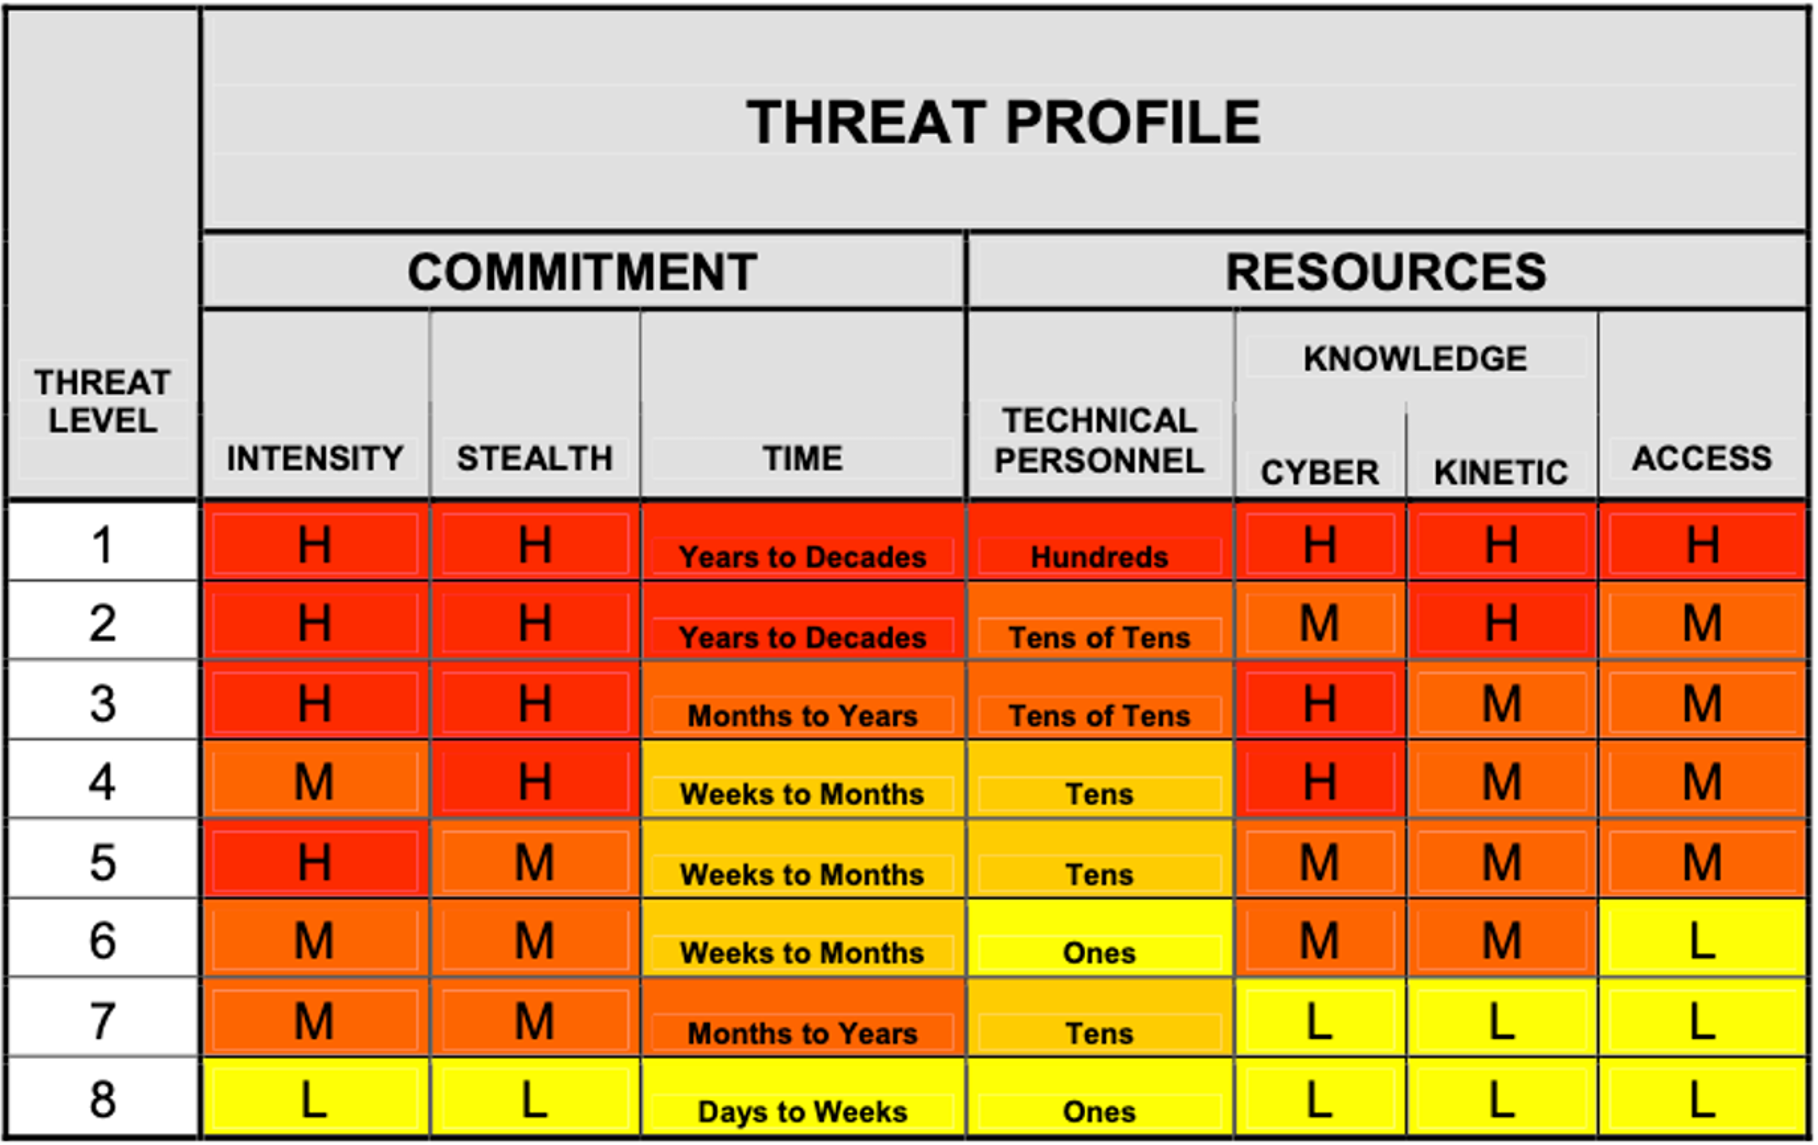
\includegraphics[width=1\textwidth]{images/Threat_Profile.png}
	\caption{Threat Profile \protect\cite{woodard2007categorizing}}
	\label{fig:APTAttribution-codebase}
\end{figure}

The commitment attribute family is used to quantify a threat’s drive and willingness to pursue a goal.  The threats with the highest level of commitment will stop at nothing in pursuit of the end goal.   On the opposite end of the spectrum, threats with less overall commitment will be less willing to commit time and resources to this goal.  The intensity threat attribute is used to measure what a threat is willing to risk to accomplish its goal.  A High (H) level of intensity means that a threat is highly determined to pursue its goal and is willing to accept any and all negative consequences to meet it.  In contrast, a Low (L) level of intensity is not willing to accept negative consequences.  Stealth is the threat’s ability to maintain a necessary level of secrecy throughout the pursuit of its goal and range from highly capable to not capable.   The third attribute for commitment is time measured in days, weeks, months, years, and decades.  A good example of a disruptive technology that takes years to decades of planning and developing to deploy is the Stuxnet Worm.  

The resources attribute family are sets of characteristics that measure resources in the number, abilities, and access of personnel.   The technical personnel threat attribute describes the group size of technical personnel that the threat can use to pursue the goal.   The scope of this attribute is focused in specific areas of knowledge or skills, such as kinetic or cyber, and those directly involved with the actual fabrication of the group’s capabilities.  This area is broken into four levels based on number of resources and ability to communicate.  The amount of and ability for personnel to communicate is key to support innovative design and development, but this alone cannot change the speed at which innovation takes place.  The knowledge threat attribute is the proficiency of, support structure for, the threat’s capability to apply the technical personnel to the goal.  It is broken into 2 sub-categories (cyber and kinetic), with a high, medium, low rating is applied to each.  Access is the last threat attribute and can be described as the ability for a threat to place a group member within a restricted system at a specific level of access.  There are three level to this attribute, placement with unlimited access, placement with limited access, no placement.  An example of this would be the use of Close Access Teams (CAT) to provide physical access to restricted systems.

From all these data points a Threat Level can be applied that describes the capability of a threat to reaching its goal.  Threat Level 1 is the most capable, and Threat Level 8 being the least capable.  Threat Level 8 threat may be able to have the impact that a level 1 threat, but important details on characteristics, supporting infrastructure, and timing would differ that could be useful in the application of applying threat attribution.  It is impossible to capture and categorize each threat attribute with 100\% correctness, but this framework can be used to assist organizations in categorize threats using a common vocabulary. 

In review of some historical examples of attributed cyber threats and their impacts on military policy we use the generic threat matrix presented above.  In this review there will be descriptions from different times, areas, and scopes.  This is not meant to be an exhaustive survey, but a varied of examples picked over time from different areas. 

\begin{figure}
	\centering
	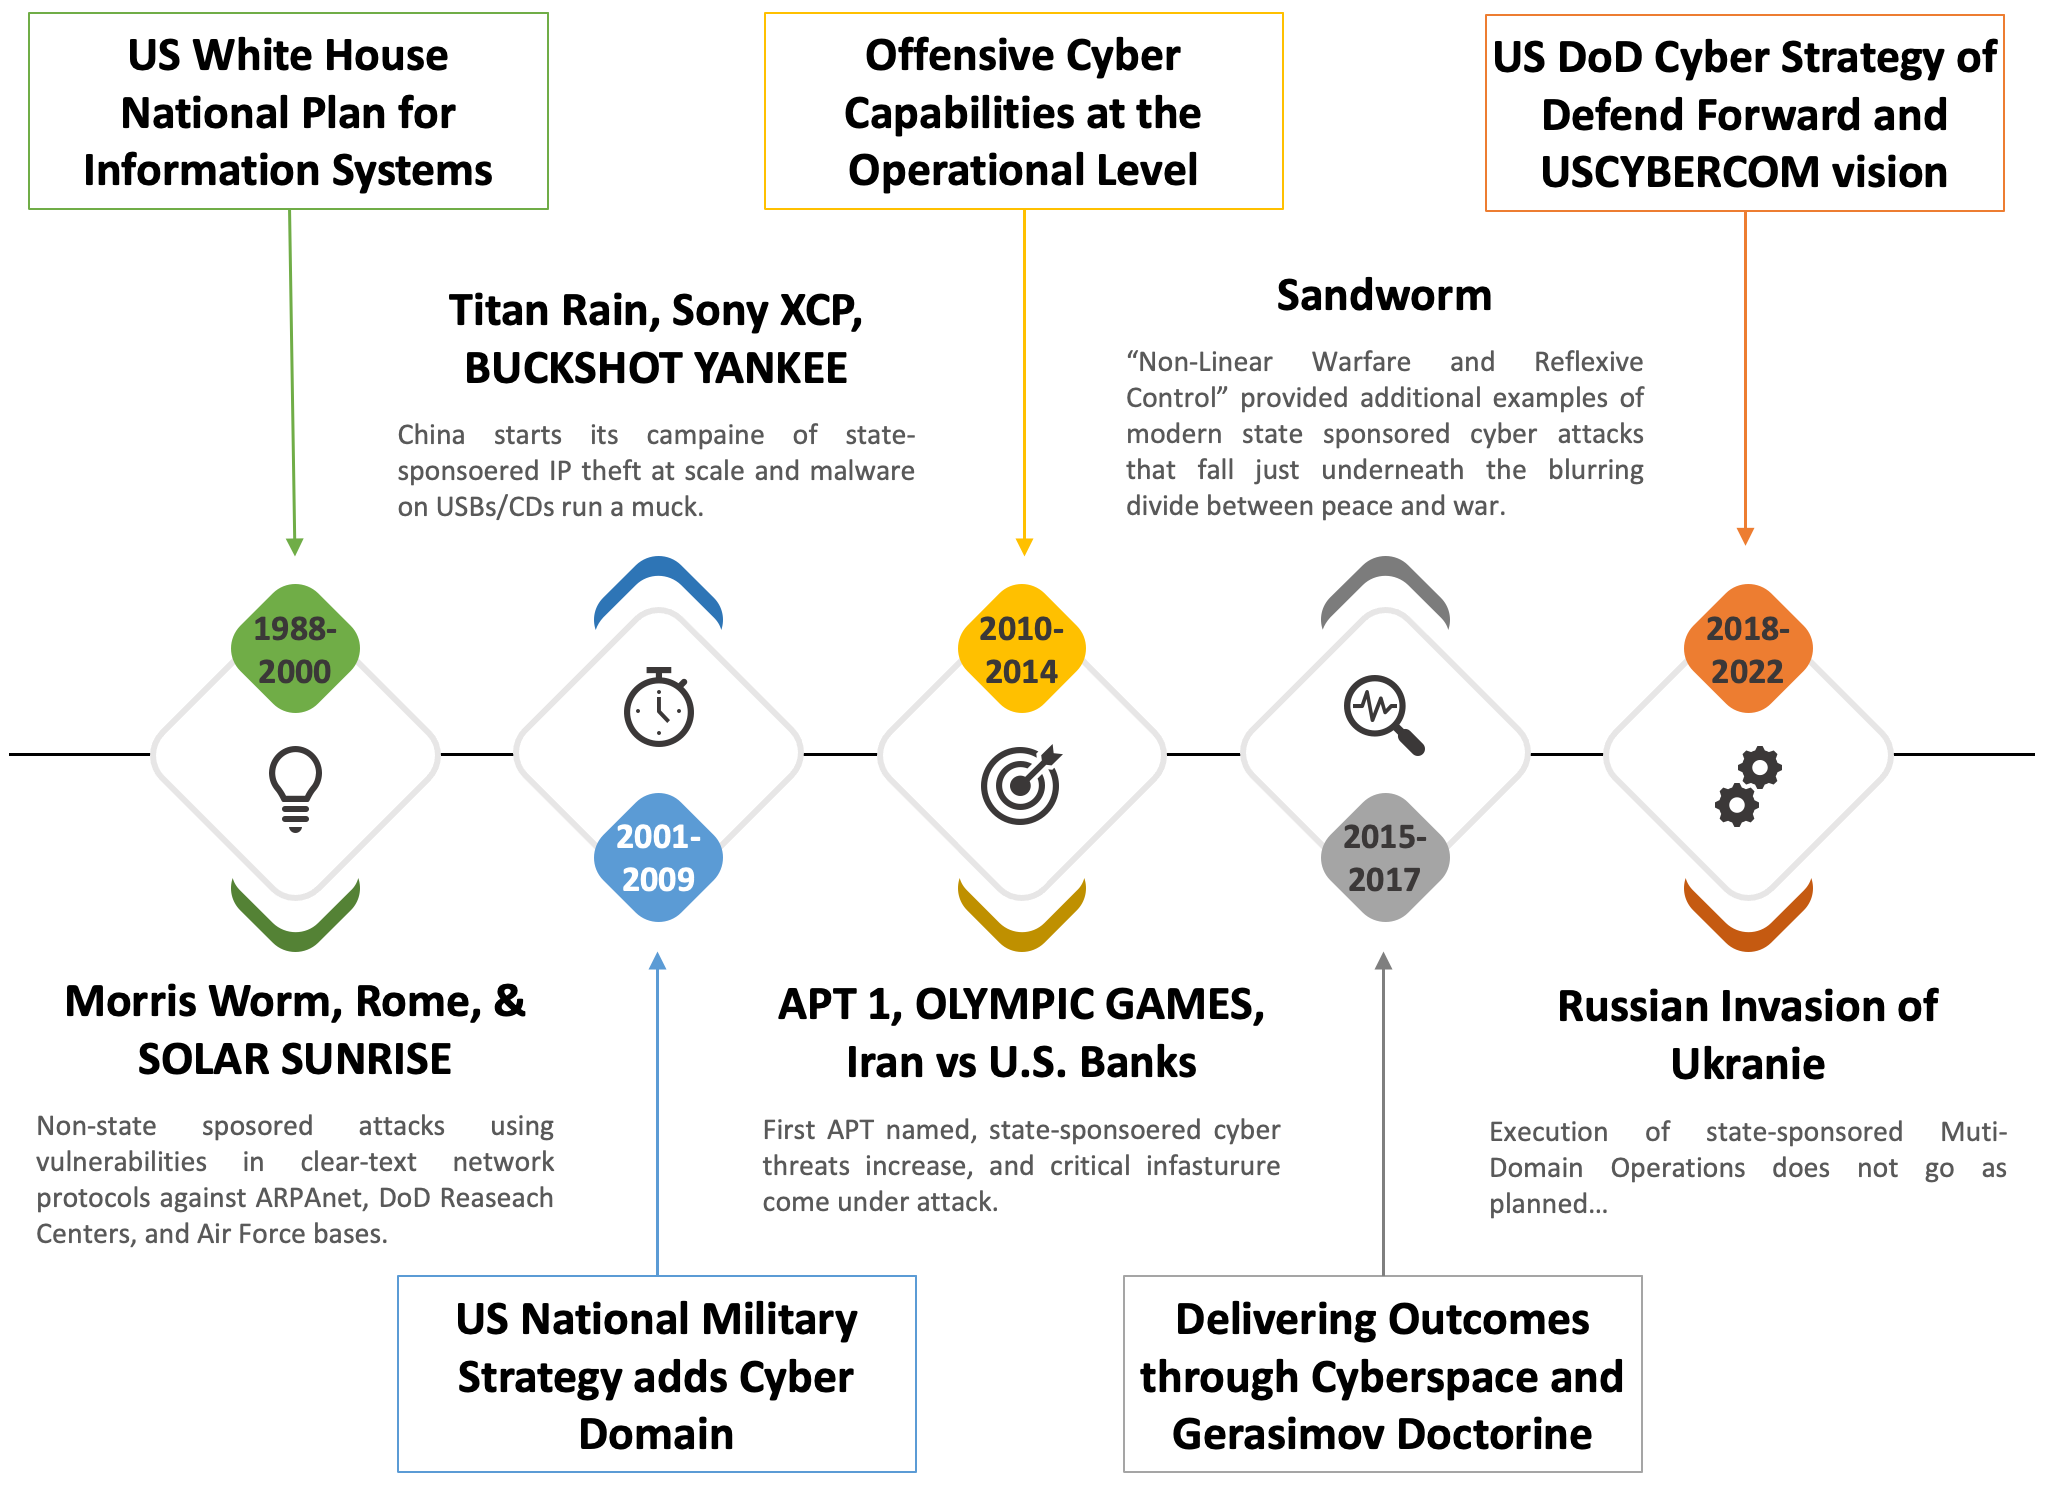
\includegraphics[width=1\textwidth]{images/Timeline1.png}
	\caption{Timeline \protect}
	\label{fig:Timeline}
\end{figure}

The Morris Worm was the work of a 23-year-old Cornell University graduate student Robert Tappan Morris Jr.  Around 8:30pm on the 2nd of November in 1988 this worm was released upon the ARPAnet from a computer at the Massachusetts Institute of Technology (MIT).  The worm contained multiple vectors to propagate from one Unix-based operating systems to another.  

These vulnerabilities included:

\begin{enumerate}
  \item A weakness in the sendmail program, which allowed the worm to send copies of itself to other computers via email.
  \item A flaw in the fingerd program, which allowed the worm to execute arbitrary code on the targeted computer and gain access to user accounts.
  \item A vulnerability in the rsh (remote shell) program, which allowed the worm to execute commands on other computers and propagate itself further.
  \item A weakness in the password file system, which allowed the worm to bypass authentication and gain access to user accounts.
\end{enumerate}

These vulnerabilities were not new, but the Morris worm was one of the first instances where they were exploited in a coordinated attack.  The speed at which this happened was at the time unprecedented.  Within 24 a hour time frame, an estimated 10\% of the computers that were then connected to this network had been hit with it, around 6,000 of the 60,000 total at the time.  The article in the New York Times that describes the incident was the first time that this periodical used the term “ the internet” to describe the international group of computer communications networks that the worm used to propagate.  Another interesting point about this event is that Mr. Morris’s father was the chief scientist for a computer security arm of the National Security Agency.  

Attribution for this attack was easily obtained through a combination of technical analysis and investigation by law enforcement agencies.  Investigators were able to track the origin of the worm to a computer at MIT, which was owned by Morris. They also found evidence that Morris had tried to cover his tracks by modifying the code to remove references to his name and by using several different computers to launch the worm. Technical analysis of the worm's code also revealed that it contained a flaw that caused it to spread more rapidly than intended, which further implicated Morris as the creator.  Morris eventually confessed to creating the worm and was convicted of violating the Computer Fraud and Abuse Act, becoming the first person to be prosecuted under the law.  Specifically within the technical analysis, investigators at the Defense Advanced Research Projects Agency (DARPA) were able to analyze the network traffic generated by the worm and trace it back to its source.  In addition to the technical analysis, investigators also conducted interviews with Morris's colleagues and acquaintances, which provided additional evidence linking him to the creation of the worm. Morris's own behavior, such as his attempts to cover his tracks and his evasiveness when questioned by investigators, further suggested his involvement in the creation of the worm.  The threat profile using the generic threat matrix was an 8, because of the low characteristics associated with stealth, time, number of technical personnel, and access.  \cite{brassardmorris}  

In March 28th of 1994, system administrators at Rome Air Development Center, Griffiss Air Force Base in New York (Rome Labs) discovered their network had been penetrated and compromised using telephone modem connections.  Initially, seven systems were found to be a part of the initial compromise that had a sniffer program installed on them that aided the attackers in gathering over 100 valid user account credentials.  These credentials were used in the next 26 days to provide access to data on systems with in the US Air Force, Army, Navy, NASA, NATO, and even the South Korean Atomic Research Institute.     

A compromise of this size of the defense industrial based had not been seen up to this point and was executed by two attackers with commercial off the shelf equipment.  The hacker known online as the “Datastream Cowboy” was a 16 year old from the United Kingdom.  He commonly used an internet provider based out of New York, mindvox.phantom.com, to establish a connection with Rome Labs.  In order to mask his connection he frequently routed his communications through systems in multiple countries in Europe, South America, and Mexico.  Datastream had launched these attacks with only a 25 MHZ, 486 SX desktop computer with a 170 Megabyte hard drive.  This is a modestly powered system with limited storage capacity when compared to other consumer grade equipment at the time.

The second attacker, Kuji, was a far more sophisticated hacker than the 16 year old Datastream Cowboy.  It took investigators more than two years after Datastream Cowboy’s arrest to apprehend Matthew Bevan, the 21-year-old son of a local police officer.  Kuji appears to have tutored Datastream Cowboy on how to break into networks and on what information to obtain.  If an attack that Datastream Cowboy was conducting on a system failed in gaining him access, he would commonly engage in a 20-40 minute on-line "chat sessions" with Kuji.  Following the on-line conversation, Datastream Cowboy was observed attack the same system again, but this time succeed.  In return for mentoring Kuji commonly received a copy of the data the accessed.  After Datastream Cowboy was apprehended, he told investigators that he had never physically met Kuji and only communicated with him through the Internet or on the telephone.  When interviewed, Kuji said that he was motivated by gaining “any information I could find relating to a conspiracy or cover-up of the UFO phenomenon.”  Additionally, he said he was bullied in school and the hacking world was pure escapism for him.  

Attribution for this attack required coordination between US DoD and UK authorities.  The combination of technical analysis, forensic investigation, and law enforcement cooperation was needed to enable attribution.  Firstly, investigators were able to trace the origin of the attacks to computers and networks associated with the two individuals. They also found evidence that the attackers had used a variety of hacking techniques and tools to gain unauthorized access to the Rome Labs network and exfiltrate sensitive information.  In addition, forensic analysis of the compromised systems provided further clues as to the methods and techniques used by the attackers.  One key piece of evidence that led investigators to Datastream Cowboy was his use of a specific hacking tool called "QAZ Trojan". This tool was found on the compromised systems at Rome Labs and was also used in other attacks that were attributed to Datastream Cowboy. Investigators were able to analyze the QAZ Trojan and identify unique characteristics that allowed them to link it to the same individual.

The QAZ Trojan had a number of capabilities that made it a powerful tool for hackers. These included:

\begin{enumerate}
  \item Backdoor access: The Trojan provided a backdoor into a compromised system, allowing an attacker to access the system at any time without the user's knowledge.
  \item Remote control: The Trojan allowed an attacker to remotely control a compromised system, including executing commands, uploading and downloading files, and modifying system settings.
  \item Keylogging: The Trojan was capable of logging keystrokes, which allowed an attacker to capture passwords and other sensitive information.
  \item Screen capture: The Trojan could take screenshots of a compromised system's desktop, which allowed an attacker to monitor the victim's activities.
  \item File transfer: The Trojan allowed an attacker to transfer files to and from a compromised system, which could be used to exfiltrate sensitive data or upload additional malware.
\end{enumerate}

A key piece of evidence that led investigators to Kuji was his use of a specific hacking tool called "Vorpal".  This tool was found on the compromised systems at Rome Labs and was also used in other attacks that were attributed to Kuji.  Investigators were able to analyze Vorpal and identify unique characteristics that allowed them to link it to the same individual.

Secondly, law enforcement agencies were able to gather intelligence on the activities of Datastream Cowboy and Kuji through their cooperation with foreign law enforcement and intelligence services. Both individuals were eventually arrested and charged with computer-related crimes, which further solidified the attribution of the attacks to them.  Intelligence was gathered on both hackers activities and online presence.  They identified online forums and chat rooms where they communicated with other hackers and discussed their activities. They also traced their use of various online pseudonyms and aliases, which helped to build profiles of their online activities.  The threat profile using the generic threat matrix was an 6, because of the characteristics associated with stealth, intensity, number of technical personnel, and access.  \cite{delibasis2007modern}

The pattern of successful computer intrusions executed against the DoD by small groups of non-state-sponsored hackers sprinkled across the planet did not stop with the Datastream Cowboy and Kuji.  A common theme within successful network intrusions at this time was the use of known vulnerabilities to exploit systems and the blanketed use of clear text network authentication protocols that enabled attackers to propagate across shared networks quickly.  Typically, these attackers manually exploited systems using low to medium level cyber threat techniques.  

This pattern continued and in January of 1998 tensions escalated between the United States, the United Nations, and Iraq because of the recent expulsion of UN weapon inspectors by Saddam Hussein.  On Feb 3rd and 4th root-level compromises were detected across multiple US Air Forces Bases within the continental united states that was called SOLAR SUNRISE.  The cyber-attack managed to get access to more than 500 computers which belonged to the US military, US government, and private defense sector.  In the attack the hackers used a virus against systems running the Solaris operating system.  At this point in time there was no known virus found on the Solaris or SunSolaris systems and this was the first attack of its kind against this operating system.  The vulnerability that the attackers used to gain an initial foothold was a known \emph{rpc} vulnerability called \emph{statd}.  This vulnerability allowed the attackers to remotely execute arbitrary commands of their choice using the privileges of the statd service.   From there the attackers installed backdoors, keyloggers, and network sniffers to enable persistent and additional access to systems.  

This computer hacking incident quickly turned into a multi-agency effort that saw unprecedented interagency cooperation between the Army, Navy, Air Force, FBI, NASA, CIA, NSA, and others.  This unusual level of cooperation quickly resulted in the DoJ being able to obtain nine court orders in fewer than 10 days and a Title III wiretap that was approved in one day.  In the end, this attack was not executed by Iraqi state-sponsored hackers, but two 16 year old hackers from Northern California and an 18 year old from Israel.  They named themselves as “the Analyzers” and this incident gave the very first nation state level cyber-war alarm which proved to be nothing but a false-alarm.  The investigation that led to the attribution of the Solar Sunrise attack to three teenagers, two from California and one from Israel, involved a combination of technical analysis and law enforcement techniques.  The investigation was led by the US Air Force Office of Special Investigations (AFOSI) and involved collaboration with other US government agencies.  Investigators used a range of techniques to trace the attack back to its source, including analyzing network traffic, examining logs and other forensic evidence, and interviewing personnel who may have had knowledge of the attacks.  A key breakthrough in the investigation came when investigators discovered that one of the attackers had used a personal email address that was associated with his real name.  This led investigators to identify the individuals responsible for the attack as Dhananjay "Jay" R. Desai and Aaron D. Hesse, both from California, and Ehud "Tim" Tenenbaum from Israel.  The attribution of the Solar Sunrise attack to these three individuals was seen as a significant achievement in the field of cyber-investigations, as it demonstrated that even sophisticated attacks on government computer systems could be traced back to their source and that perpetrators of such attacks could be held accountable for their actions.  Discovering of this kind of vulnerability forced US Defense department to take strong steps to avoid such thing in the future.  \cite{purohitcyber}  The threat profile using the generic threat matrix was an 8, because of the characteristics associated with stealth, intensity, number of technical personnel, and access.

While the 42nd President of the United States was in office in January of 2000, the White House published a unclassified paper titled “Defending America's Cyberspace: National Plan for Information Systems”.  A key motivation for publication of the plan was to facilitate public-private sector cooperation on information systems protection. This plan outlined a number of defensive milestones and accomplishments, but did not address the application of offensive network capabilities to the DoD or applying attribution to attacks against information systems. \cite{cip-plan:2000}  

In 2003, before cyberspace was declared to be a war fighting domain, there was a series of attributed computer network intrusions labeled TITAN RAIN that US Defense Department investigators believed to have originated from the People’s Liberation Army of China.  These series of intrusions marked a turning point for the DoD in which the attributed activities were shown to have not been conducted by any free-lance hackers but long term operations conducted by state-sponsored hackers.  The sensitive information that was gained from this series of attacks came from a variety of US defense contractor computer networks, Sandia National Laboratories, US Army Space and Strategic Defense Command, FBI, NASA, and the United Kingdom’s Ministry of Defense.  The attribution of the cyber threat attacks called TITAN RAIN was based on a combination of technical analysis, intelligence gathering, and collaboration between multiple organizations.

Some of the key information that aided in the attribution of the attacks included the following.

\begin{enumerate}
  \item Technical indicators: Analysts identified a set of unique technical indicators associated with the TITAN RAIN attacks, such as specific malware samples, command-and-control infrastructure, and methods of exploitation.
  \item  Network traffic analysis: Investigators analyzed network traffic logs from affected organizations to identify the source of the attacks and the tactics, techniques, and procedures used by the attackers.
  \item Intelligence gathering: Intelligence agencies used a range of sources and methods to collect information about the identity and location of the attackers, including human intelligence, signals intelligence, and imagery intelligence.
  \item Collaboration between organizations: Multiple organizations, including the FBI, the National Security Agency (NSA), and private security firms, worked together to share information and coordinate their efforts in investigating the attacks.
  \item Attribution to specific threat actors: Ultimately, the TITAN RAIN attacks were attributed to a group of Chinese state-sponsored hackers known as the "Byzantine Candor" group, based on a combination of technical and intelligence analysis.
\end{enumerate}

In a similar vein to the Chinese government's response to the Mandiant report in 2010 and 2013, China refuted the charges of being involved in the TITAN RAIN attacks and suggested instead that the network security of Chinese computers and websites were lacking in such a severe way that they could have been exploited by any random hackers across the world.  This was a convenient answer, but did not line up with evidence of the size, complexity, patience, coordination, discipline, and professional manner in which the attacks were carried out.   The Director of Research of SANS Institute at the time, Adam Paller, stated that “the attacks were from individuals with intense discipline and no other organization except military could do this”.  \cite{titanrain2016}

This was a key turning point in the domain of cyber and how threats influenced military strategy across the globe.  The era of advanced persistent threats began and nation-states started building resources to gain enhancing capabilities in this area to assist in a variety of national priorities that ranged from areas of intelligence, military capabilities, economic growth, and gaining geo-political status.  The threat profile using the generic threat matrix was an 3, because of the intense application of resources and level of commitment that was not common place at the time.

In the 2004 National Military Strategy, the Chairman of the Joint Chiefs of Staff Richard Myers declared cyberspace a “domain” of conflict alongside the air, land, sea, and space domains.  \cite{myers2004national}  It was noted that the US DoD must maintain its ability to defend against and to engage enemy actors in this new domain.  That same year the Secretary of Defense Donald Rumsfeld divided Joint Task Force – Computer Network Operations (JTF–CNO) into defensive and offensive components.  \cite{dod2011strategy}  The component that held the responsibility for defense of the cyberspace domain was the Joint Task Force – Global Network Operations (JTF–GNO) and the component that held the responsibility for offensive cyberspace operations planning was the Joint Functional Component Command – Network Warfare (JFCC–NW).

The commercial company Madiant started to provide detailed reporting on what it called Advanced Persistent Threat (APT) 1 in 2010.  The position of Mandiant was that “The Chinese government may authorize this activity, but there’s no way to determine the extent of its involvement.”  That changed in 2013 when they reported that now we have the evidence required to change our assessment to say that the groups conducting these activities are based primarily in China and that the Chinese Government is aware of them.  \cite{APT1Mandiant2013}  In response to this update, the Chinese Defense Ministry provided this “It is unprofessional and groundless to accuse the Chinese military of launching cyber attacks without any conclusive evidence.”  \cite{lewis2005computer}

Operation BUCKSHOT YAHKEE was a response plan executed in 2008 to clean up a worm from DoD networks called agent.btz.  Unlike earlier worms described in this survey, the primary means of propagation this worm leveraged the windows auto-run feature and the abundant use of usb thumb drives to move data between systems.  Agent.btz was variant of the SillyFDC worm that had been observed being used by Russian hackers before.  Some of its capabilities included abilities to scan computers for data, open backdoors, and send through those backdoors to a remote command and control server.  One unique feature of SillyFDC is its ability to modify its code and behavior in response to changing system conditions. For example, it can detect if it is running in a virtual machine environment and modify its behavior to avoid detection.  This family of malware was unique in that it also attempted to disable antivirus software and other security measures on the infected system, making it more difficult to detect and remove.  The agent.btz worm was particularly challenging to detect and remove due to its use of advanced encryption techniques to hide its activity and evade traditional antivirus and security tools. It was also designed to remain dormant for extended periods, allowing it to evade detection and continue to spread across networks.  It is believed that initial infection was facilitated by a foreign intelligence agency that left an infected thumb drive in the parking lot of a DoD base in the Middle East.  From there it to was observed spreading across unclassified and classified information systems at US CENTCOM.  Attribution of the agent.btz worm being used against CENTCOM is not entirely clear, but it is believed to have been the work of a foreign intelligence agency, possibly Russia or China.  This incident highlighted the vulnerability of even the most secure military networks to sophisticated cyber attacks.

Three years before this, in 2005 Sony BMG had found itself in trouble becasue of the development and opperational use of the windows auto-run feature and a piece of Digital Rights Management (DRM) software called the Extended Copy Protection (XCP) rootkit.  Sony had been losing revenue because of peer-to-peer file sharing software.  Statements by Sony Pictures Entertainment US Senior VP Steve Heckler foreshadowed these events when he told attendees of the Americas Conference on Information Systems in 2000 that "The industry will take whatever steps it needs to protect itself and protect its revenue streams... It will not lose that revenue stream, no matter what... Sony is going to take aggressive steps to stop this. We will develop technology that transcends the individual user. We will firewall Napster at source – we will block it at your cable company. We will block it at your phone company. We will block it at your ISP. We will firewall it at your PC... These strategies are being aggressively pursued because there is simply too much at stake."  The combination of this aggressive stance and Sony’s application of a malicious software in their products did not help their cause. 

The DoD did not effectively learn from Sony’s mistake, but did take measures to clean the infection and install security controls to help ensure this particular attack method was mitigated going forward.  The it took the Pentagon nearly 14 months to intercept the covert channel that this worm used and clean the infection from military networks.  Many changes were implemented in terms of people, processes, and technology that directly effected American military strategy and good deal of lessons were learned in having better situational awareness of military networks.  The threat profile using the generic threat matrix was an 8, because of the characteristics associated with stealth, intensity, number of technical personnel, and access, but to this date public attribution has not been confirmed.  \cite{lynn2010defending}

In June of 2009, the Iranian nuclear power enrichment plant in Natanz came under attack by an updated version of what would be called the world’s first digital weapon, Stuxnet.  In a similar lane to the Agent.btz worm, Stuxnet used usb thumb drives as the primary prorogation method, but the similarities in commitment towards the goal and resources applied stop there.  \cite{zetter2014countdown}  This worm was designed to target industrial control systems, specifically those used to control centrifuges at an Iranian nuclear facility. The complexity and sophistication of the worm led many experts to believe that it was the work of a nation-state.

The primary differences in the commitment and resources attribute families project a sharp contrast from previous references in this survey.  Evidence in the amount of time that this piece of malware was under development can date back to around 2005.  Lines of code is also a significant outlier when compared to other malware samples collected within the same time frame.  Sophos, a cybersecurity company specializing in malware analysis and enterprise security occasionally publishes some of their analysis on trends found within malware.  In 2010  the analysis provided by Sophos in this area described most malware contained around 125 lines of code.  Stuxnet was shown to contain more than 15,000 lines of code.  Another significant difference was the use of 4 different zero day vulnerabilities used to get the malware to its intended destination. 

Direct public attribution has not been definitively verified, but most researchers agree that the evidence points to a collaborative effort by the US and Israeli governments within Operation Olympic Games.  It has been reported that the development of Stuxnet began under the George W. Bush administration and continued under the Obama administration.  The operation is considered a landmark in the history of cyber warfare, as it demonstrated the potential for cyber attacks to cause physical damage to critical infrastructure.  The threat profile using the generic threat matrix was an 1, because of the unprecedented characteristics associated with stealth, intensity, time, number of technical personnel, access, and kinetic effect that the Stuxnet worm had.  \cite{kaminski2020operation}

In response to the Stuxnet worm and ongoing economic sanctions the Iranian government made a retaliating strike on the US.  In another turn of events that seems to be a modern trend for state-sponsored cyber attacks, this attack was pointed not to the Israeli Mossad, the US Central Intelligence Agency, or the US military, but instead they attacked important pieces of gray space critical infrastructure, including banks, oil manufacturing, and cellular service providers.  

In Feburary of 2012 the Director of National Intelligence James R. Clapper Jr. told the US Congress that “Iran’s intelligence operations against the United States, including cyber capabilities, have dramatically increased in recent years in depth and complexity.”  Specifically, Iran’s Ministry of Intelligence and Security and a special unit within Iran’s Revolutionary Guard Corps called the Quds Force are suspected of carry out this and other attacks against critical infrastructure.  Most of these attacks were simple distributed denial-of-service attacks designed to overload an organization’s web site and block legitimate access to the servers.  The threat profile using the generic threat matrix was a 7, because of the characteristics associated with stealth, intensity, number of technical personnel.

The Center for Strategic \& International Studies (CSIS) and Georgia Tech Research Institute (GTRI) published a pap er in 2013 titled “Offensive Cyber Capabilities at the Operational Level, The Way Ahead”.  The paper examines in greater depth whether the Defense Department should make a more deliberate effort to explore the potential of offensive cyber tools at below that of a combatant command.  It details the growing need for offensive cyber capabilities at echelons below Combatant Commands (COCOM)s and the struggle of limited resources, lack of understanding of the capabilities, proper conditions of use, not well-developed requirements, and immature tool sets.  In the end this paper presents the opinion of “At present, neither the procedures nor the tools are sufficiently robust to merit a delegation of offensive cyber authorities beyond the very limited ways in which they have been utilized thus far.”  \cite{nakashima2012iran}

A research paper published by the NATO Defense College in November of 2015 titled “Russia’s Renewed Military Thinking: Non-Linear Warfare and Reflexive Control” provided additional examples of modern state-sponsored cyber attacks that fall just underneath the blurring divide between peace and war in the 21st century threat landscape.  In this paper, evidence of the adoption of the “Gerasimov Doctrine” is presented.  Additionally, the book SANDWORM by Andy Greenberg provides a detailed timeline of cyber attacks executed by the Kremlin.

To support this new shift in military doctrine, General Valery Gerasimov, the Chief of the General Staff of the Russian Federation’s Armed Forces, argues that “the role of non-military means of achieving political and strategic goals has grown, and, in many cases, they have exceeded the power of force of weapons in their effectiveness.”  The doctrine describes ways Russia is leveraging cyber attacks and organizing resources within unified informational spheres towards their mission goals.  Examples of these efforts are the state-sponsored attacks against Estonia and Georgia that support Russia’s goal of necessary expansionism.  The threat profile using the generic threat matrix was a 5, because of the characteristics associated with stealth, intensity, and balance between cyber/kinetic/access that aligns with the Gerasimov Doctrine.  

The cyber attack referred to as the NotPetya worm is an example of the greater level of need for advancing software forensic tools in order to better help determining adversarial attribution.  The NotPetya worm was created by a group of Russian military intelligence hackers known as Sandworm, and was intended as a climactic strike against Ukraine in the years-long cyberwar Russia had carried out against its southwestern neighbor.  This worm presents an interesting case because of the unique combination of using stolen National Security Agency hacking capabilities, an open-source credential-harvesting tool called \emph{Mimikatz}, and the hijacking of a update system within a common piece of Ukrainian accounting software that was used used by practically every company that filed taxes or had business ties in the country.  \cite{greenberg2018untold}

This lowering of resources needed to build and integrate this capability, in combination with nation states conducting advanced offensive cyber operations, in different instances, at scale and with precision, below the threshold of traditional war requires new ways of thinking.  Specifically, when focusing in on the previous history of applying cyber threat attribution either incorrectly or not in a timely manner, there is significant risk to critical infrastructure.  New ways of applying attribution in this domain is required.  Within this timeline of events there are opportunities for advancement within the areas of analysis that can be automated and correlated for the benefit of accuracy in cyber threat attribution.  

Current US policy for conflicts in the cyber domain is an evolving area that include a number of key stakeholders.  US Cyber Command (USCYBERCOM) released an updated vision in April of 2018 that built upon the USCYBERCOM commander’s vision released in 2015.  The vision in 2015 was titled, Delivering Outcomes through Cyberspace.  The updated vision described the growing need, dynamic nature, and interconnection between cyber and other warfighting domains.  “The cyberspace domain that existed at the creation of US Cyber Command has changed. Our adversaries have exploited the velocity and volume of data and events in cyberspace to make the domain more hostile.”  A key point of this change lies within what is described as a new normal way of interacting with the United States in cyberspace.  Adversaries continuously operate against the US below the threshold of armed conflict without fear of legal or military consequences.  Similar issues with cyber threat attribution are still present in 2018 that Madinat attempted to overtly call out in 2010.  \cite{uscybercom2018vision}

\begin{comment}
In September of 2018 the DoD released it’s cyber strategy that within page one of the summary calls out the strategic competition in cyberspace between the US, China, Russia, North Korea, and Iran.  This approach outlined five specific lines of efforts lines of effort.  /\cite{rugge2018cyberspace}

\begin{enumerate}
  \item build a more lethal force
  \item compete and deter in cyberspace
  \item expand alliances and partnerships
  \item reform the Department
  \item cultivate talent
\end{enumerate}

\end{comment}

An important shift in focus of this document was apply the concept of “defend forward” in order to disrupt or halt malicious cyber activity at its source, including activity that falls below the level of armed conflict.  This is a step in the right direction to help create policy that better address state-sponsored cyber threat actors attack on gray space infrastructure, but greater levels of focus are needed on policy and efforts for the DoD to better apply attribution to cyber threats and provide Offensive Cyber Capabilities at the Operational Level.  \cite{goldsmith2022united}

In July of 2019 there was a hearing to consider the nomination of General Mark A. Milley to be the Chairman of the Joint Chiefs of Staff at the 116th US Congress.  Within this nomination hearing there were many questions related to cyber threats and the change from a counter-insurgency focused military to a near-peer battle.  Chairman of the Senate Armed Services Committee, U.S. Sen. Jim Inhofe set the stage with “The National Defense Strategy makes it clear that strategic competition with China and Russia, not terrorism, is now our primary national security concern.  China and Russia have passed us in key areas and are catching up with others.”  This are key points of reference regarding the change in military strategy and in influence the cyber domain has in modern military.  When General Milley was asked questions on the theory of deterrence within the cyber domain, a parallel to a particular phase of American football was used, “a good offense is critical and that is the best defense”.  

This emphasis on the lethality of the U.S. military’s offensive capabilities, especially in the context of the “defend forward” concept is concerning because it still suffers from similar drawbacks that CSIS and GTRI report outline in 2013.  To overmatch and disrupt or halt malicious cyber activity at its source, attribution needs to be better addressed and capabilities need to be pushed towards the tactical edge to maintain superiority in the cyberspace domain.  Russia’s invasion of the Ukraine in February of 2022 illustrates the interseation of modern warfare domains.  There could be a great number of reasons for this result to be taking place.  On March 8th, 2022, during a House Permanent Select Committee on Intelligence hearing on worldwide threats, Director of the Central Intelligence Agency William Burns describes four false assumptions that the Russian dictator has made:  

“First: That Ukraine, in his view, was weak and easily intimidated. Second: That the Europeans, especially the French and Germans, were distracted by elections in France and a leadership succession in Germany and risk averse. Third: He believed he had sanctions-proofed his economy in the sense of creating a large war chest to foreign currency reserves. And fourth: He was confident that he had modernized his military and they were capable of a quick, decisive victory at minimal cost." 

The fourth assumption plays a key role in potentially applying assistance in what and how a modernized military need operate to be prepared for a conflict with a near-peer.  For the U.S. DoD to defend froward and apply overmatch with cyber in this new normal environment, research is needed to investigate our ability to apply cyber threat attribution.  Improved performance of software forensics utilizing multi-dimensional analysis to detect semantic differences between known and unknown cyber threat actors can assist in this endeavor of better applying authorship attribution.

\begin{comment}
Shadow Brokers, EternalBlue, EternalRomance
    ETERNALROMANCE is a SMB1 exploit over TCP port 445 which targets XP, 2003, Vista, 7, Windows 8, 2008, 2008 R2, and gives SYSTEM privileges (MS17-010)
    ETERNALBLUE is a SMBv2 exploit for Windows 7 SP1 (MS17-010)

WannaCry ransomware used this exploit to attack unpatched computers.
\end{comment}

\begin{comment}
The Stuxnet worm is an example of the greater levels of need for advancing software forensic tools in determining adversarial attribution. \cite{parker2011stuxnet}  One area of Stuxnet was the use of a modified Step7 library file, named s7otbxdx.dll, to communicate with a Siemens Programmable Logic Controller (PLC) (see Figure \ref{fig:stuxnet-modified-s7otbxdx.dll}).  

\begin{figure}
	\centering
	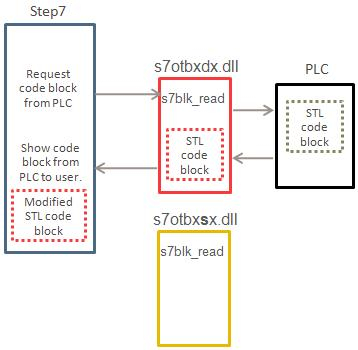
\includegraphics[width=0.5\textwidth]{images/modified_Step7.jpg}
	\caption{Stuxnet’s modified s7otbxdx.dll file \protect\cite{falliere2010exploring}}
	\label{fig:stuxnet-modified-s7otbxdx.dll}
\end{figure}

Stuxnet's modified s7otbxdx.dll forwards 93 of the original 109 exports to the real DLL, renamed to s7otbxsx.dll, for processing.  16 exports were intercepted by the custom DLL in order to modify data being sent to or returned from the PLC without the operator of the PLC realizing it. It is also through these routines that Stuxnet was able to hide malicious code on the PLC itself.
\end{comment}

In order to use software forensics to track advancing threats like that of NotPetya, the software forensics engineer needs to break the inputs into objects suitable for comparison and apply structure to these objects.  This structure can then be used to determine which objects exist across various versions and which do not.  This is not a simple task since the differences in high-level language constructs and structure, including code comments, are commonly not found in the compiled versions of the malicious software.  Techniques used to identify the fingerprints of malicious software authors come from a variety of sources and modern authorship identification techniques can be used to highlight patterns.  Previous methods of manual analysis do not meet the scale of which current malware is being manufactured.

\section{Single Dimensional Software Correlation}
Single Dimensional Software Correlation takes a single input source and uses that source to as its basis for analysis.  Historically this in combination of traditional investigative work is how advanced cyber threats are identified and tracked.  This method of correlation is a time consuming and labor intensive task of a few subject matter experts.  Depending on the experience and skill of the analysts, accuracy can be very high, but does not scale and can be influenced though the placement of false flags.  Some parts of this analysis can be automated, other parts are not easily automated.  This analysis determines the similarity of source or binary code, by comparing raw text, cryptographic hashes, and tokens.  The result is a single measure that indicates the degree of similarity.  This measure is not accurate enough to be admissible in court of law because they are not definitive.  Questions arise because the algorithms can be fooled by, for example, simple substitutions in the code with representative fixes.  Similarly, the problem of instruction reordering can be solved though grouping using the variable tracing and sorting method \cite{oh2009fight}.  Relevant methods used in authorship attribution research are referred to as stylometry.  Authorship Attribution of text of literary works offer a wide array of different techniques to identify the author of a peice of work based on a set of textual features that quantify their writing style. \cite{stamatatos2009survey} The quantified representation of this style can be viewed as a fingerprint.

As example of the inverse of the open problem of plagiarism, authorship attribution of malware is a closed-world problem that we do not typically have the source code of the software that we can easily compare the original inputs from \cite{kalgutkar2019code}.  This leaves researchers with a binary representation to inspect and as such, binary code retains very few of the surface characteristics of the original source code.  The primary focus of research in recent years has shifted toward the analysis of stylistic features of program binaries \cite{chouchane2013detecting,rosenblum2011wrote,rosenblum2010extracting}.  Usually a single dimension of software correlation will be either static or dynamic analysis of the compiled binary.  Features collected from static analysis of binaries have been shown to be useful in cases where already identified fingerprints have been found.  Features collected from dynamic analysis have been shown to have utility in cases where unknown fingerprints are collected.  Additionally, the ability to collect various types of features are specific to static or dynamic analysis.  

\cite{zeidman2012detecting} developed algorithms that look at the basic elements of code in order to find which elements are correlated to each other.  He proposes an algorithmic method that extracts program elements that are common in the samples being compared.  These methods keep each of the data structures that are found to have entries corresponding to program elements of a distinct program element type represented by program strings or program identifiers.   From that, elements are extracted based on a program object code file using a text converter to transform the program object code to text sequences by solely determining byte-by-byte whether the sequences represent characters.  Then a calculation of a correlation score based on the similar entries is done that is comprised of a number of similar strings and a number of similar identifiers.

\begin{comment}
The major drawback to this work is the high number of false positives that result from the comparison.  Efforts to improve accuracy included interpreting the elements being compared to eliminate reasons for correlation unrelated to copying, such as common algorithms, third-party code, common identifier names, common author, and automatic code generation.

DU Comment = citation(s) needed
\end{comment}

Another single dimensional software correlation technique is analysis of human readable strings in the code.  Once analysis has been performed using a single dimension procedure, an analyst then looks at subjective evidence such as comments in the code or non-obfuscated function calls.  Fake copyright notices, open source notifications, or programmer names added to source code after copying took place, in order to disguise the copying, are not uncommon in real-world cases of code theft \cite{sfbook:2011}.  Challenges arise in the ways that human readable strings can be analyzed using natural language of malware.  An automated means to understand the intent of these strings, even when armed with the latest Natural Language Processing (NLP) techniques, can be only so useful \cite{artsci:2015}.  Extracting human readible strings from compiled code can contain a rich amount of information that support the identification of authorship for known threats, but do not excel at identifying unknown threats.  Another strong area of analysis that can be gained from the extraction of string for a compiled binary are information on the toolchain providence.  Toolchain providence aims to highlight the process of tracking how the source code got turned in a compiled binary.  The value of analysis on styrings is improved when presented with strong pieces of supplemental data.  Information such as how an organization distributes its code, details of the software development life-cycle can possibly emerge.  This gives the potential to identify the programmers who authored the code.  

There is also work being done on data sets of different programming languages (Java or C++) of varying difficulty (6 to 30 candidate authors) to demonstrate the effectiveness of the Source Code Author Profiles (SCAP) approach.  It involves analyzing characteristics of source code to identify patterns and unique attributes that can help identify the author or authors of the code. This approach takes into account various factors such as the use of certain programming languages, coding styles, and coding conventions. By analyzing these characteristics, SCAP can help identify the individual or group responsible for creating the code, which can be helpful in identifying cyber threats or potential attacks.  This is based on analysis of byte-level contiguous sequence profiles in order to represent a source code author’s style.  \cite{IFIP:2006} This method has potential to show effectiveness of the model and how it is not severely affected by the absence of comments in the source code, a condition usually met in cyber-crime cases.  

There have been several instances where the SCAP approach has been used to aid in cyber threat attribution.

\begin{enumerate}
  \item Attribution of the 2017 NotPetya attack: In 2018, the UK and US governments attributed the 2017 NotPetya attack to Russia based on evidence gathered using the SCAP approach. The UK government's National Cyber Security Centre (NCSC) analyzed the malware's source code and used the SCAP approach to link it to a specific Russian military intelligence unit.
  \item Attribution of the Lazarus Group: The SCAP approach has also been used to link the Lazarus Group to a specific North Korean research institution. In 2018, the US Department of Justice indicted a North Korean programmer who was believed to be a member of the Lazarus Group. The indictment included details of the SCAP approach being used to identify the individual based on his code and development patterns.
  \item Attribution of the Anthem data breach: In 2015, the US health insurer Anthem suffered a data breach that exposed the personal information of millions of customers. The SCAP approach was used to link the attack to a specific Chinese hacking group known as Deep Panda. The attribution was based on similarities between the Anthem attack and previous attacks attributed to Deep Panda, including the use of specific code libraries and development patterns.
\end{enumerate}

The analysis of malicious code authorship and true functionality without the assistance of the underlying source code makes single dimensional software correlation difficult and a prime target for deception.  Comparing code functionality is a difficult problem that has yet to be effectively shown by any algorithm within a reasonable time.

\section{Multidimensional Software Correlation}
Multidimensional software correlation is the process of dividing attributing features into discrete categories in order to determine which elements assist the most in attribution.  One of the key elements to applying this correlation is the ability to filter and interpret the relationships in order to find the best features and eliminate false positives.  The state of research of semantic data models being leveraged for machine learning has shown promise in helping identify similar elements for correlation.  One example of this work is the concept of traceability being applied using machine learning within safety-critical domains for source code and other artifacts using Word Embedding and Recurrent Neural Network (RNN) models to generate trace links.  RNN models use word vectors to learn the sentence semantics of requirements artifacts.  An RNN system that uses Bidirectional Gated Recurrent Units (BI-GRU) has shown promise for the tracing task.  \cite{saha2019integrating}  BI-GRU, in this instance, significantly out-performed state-of-the-art tracing methods including the Vector Space Model and Latent Semantic Indexing.   This provides us an example of a solution that leverages deep learning to incorporate artifact semantics into a novel solution. \cite{guo2017semantically}  This method stands in stark contrast to the labor intensive job of manual expert selection done by an analyst described in previous section on Single Dimensional Software Correlation.  In most modern implementations of Multidimensional Software Correlation to aid in cyber threat authorship attribution all available features are used and little manual work or checks and balances are leveraged in terms of expert selection. 

An important area of focus for addressing attribution using software correlation are the range of features available to apply efficient and effective attribution.  Research being done within the area of time-series forecasting methods for cyber attacks, from network telescopes, honeypots, and automated intrusion detection/prevention systems is limited to awareness of predesignated items within a temporal scope that can be easy to miss and hard to collect.  ``To enhance awareness about specific threats, it is vital to uncover associated and, ideally, causal factors for cyber attacks"  \cite{DBLP:journals/corr/BakdashHZMTSHD17}.  For our research endeavor, this data can be used to assist in attribution based on past observation of transit data path, means, and capabilities in combination with other features already identified using expert selection.  These supporting factors can be used in order to further judge breadth, depth, and positioning of future attacks in traditional and new environments that threats are working towards having similar capabilities that exist in client-server environments.

Accurately detecting malware signatures and anomalies aids in the process of applying attribution.  A short review of malware detection is given to draw similarities to features that can be used to guide better results within authorship attribution.  We describe this research in two main different types, syntactic vs semantic analysis.  An easy way to describe the differences in these techniques is a pattern matching approach and a trait detecting approach.

Syntactic detection of modern malware is fraught with issues, a key one being the use of self-mutating software.  A good example that describes the cat and mouse game of malware detection is syntactic analysis of payload generation and encoding capabilities of the open source exploitation framework \emph{metasploit}.  Shikata-Ga-Nai is a Japanese language phrase meaning "it cannot be helped" or "nothing can be done about it" and for many years this was an accurate description of the ability of syntactic analysis tools to trigger on this specific method of encoding that is built into the metasploit framework.  At it's core, it is a polymorphic XOR additive feedback encoder.  This encoder offers three features that provide advanced protection when combined.  First, the decoder stub generator uses metamorphic techniques, through code reordering and substitution, to produce varied output each time it is used.  This makes triggering on just the shellcode very difficult, especially if unique parameters are leveraged.  This is implemented using loops with a user definable counter.  Second, it uses a chained self modifying key through additive feedback. This means that if the decoding input or keys are incorrect at any iteration then all subsequent output will be incorrect.  Third, the decoder stub is itself partially obfuscated via self-modifying of the current basic block as well as armored against emulation using Floating-Point Unit instructions.  

APT20, a suspected Chinese nation state-sponsored threat group, leverages the Shikata-Ga-Nai encoder in their payloads.  This group has a primary focus on stealing data, specifically intellectual properties.  Other named groups include APT41 and FIN6.  APT41 has been seen using this encoder within custom developed backdoors.  APT41 is a Chinese cyber threat group that has been observed carrying out financially motivated missions coinciding with cyber-espionage operations.  The financially focused threat group FIN6 also uses this encoding method to carry out some of their missions, and they have historically relied upon various publicly available tools. These missions largely involve theft of payment card data from point-of-sale systems. 

Static Malware Detection by the use of mechanisms to detect string signatures, byte-sequences, n-grams, syntactic library calls, control flow graph and opcode frequency distribution of known malware have helped keep pace with obfuscation, but some of these measure are trait detecting approaches.  Semantic malware detection measures that examine intermediate languages have been shown to provide greater levels of resilience against the polymorphic capabilities of modern malware \cite{christodorescu2005semantics}, \cite{ranjan2016boolean}.  These methods use LLVM generators to convert machine code to simplified forms in order to aid in semantic analysis that can be leveraged in identification of authorship traits.  

\begin{comment}
Next generation malware will by be characterized by the intense use of polymorphic and metamorphic techniques aimed at circumventing the current malware detectors, based on pattern matching. \cite{bruschidetecting}
\end{comment}

Provenance, a word that originates from art, refers to the chronology of location and ownership.  A detailed provenance can be used to establish that a piece of art is not a forgery or has not been stolen.  Recently, the term provenance has also been adopted and applied to other fields, including computer science, where it refers to having knowledge of all the steps involved in producing a scientific result, from experiment design through acquisition of raw data and all the subsequent steps of data selection, analysis, and visualization \cite{provenance:2011}.

The concept of provenance can also be applied to multidimensional software correlation.  The tracing of provenance in software development has become increasingly more important to tracking vulnerabilities and threats.  Models of provenance developed from observing software during its natural life cycle can be used to educate researchers on how code evolves and mutates over time.  The relation between a large file and LOC objects is very sparse and indexing can allow the relations to mapped as clusters of LOC and their containing files.  Using these observations, an analyst is able to observe statistical trends of modifications made to files over time and see changes in sparse structures and natural growth patterns throughout a software development life cycle.  In a typical scenario, files exhibit rapid initial growth with code being added in large chunks, and then when the changes of the software are in place, small bug fixes are the majority of modifications thereafter.  By tracking the unique relationship between file size and lines of code, an analyst can map codelets as code patches with co-migratory patterns in files.  \cite{provenance2:2014}  For instance, a generative model that uses a Bayesian game to assist in Active Malware Analysis (AMA) has shown to have strong statistical results in identifying relations in software provenance between malware families \cite{sartea2020bayesian}.  

As an extension of this concept of provenance, experiments have shown benefits in the selection of informative features using genetic algorithms (GA).   Specifically, authorship attribution of social media and literary texts using machine learning methods in combination with GA has shown the ability to reduce the time costs by half in comparison with deep Neural Networks alone in comparable accuracy.  \cite{fedotova2021authorship}  In addition to an improvement of time, cost though the implementation of Neural Networks and GA, there have also been a series of comprehensive experiments that present results that significantly increase the rate of accuracy in terms of recognition.  Focusing feature selection on syntactic attributes for authorship attribution using multi-objective genetic algorithm and a Support Vector Machine (SVM) classifier has been shown to increase the recognition rate around 15 percentage points.  \cite{varela2011selecting}

Traditional grammar-based analysis techniques used to identify authors have been adapted for use in software source code (\cite{kustanto2009automatic}, \cite{lesner2010novel}, and \cite{jadalla2008pde4java}).  Code, like speech, consists of patterns that can link the author to the product.  The langage Prolog offers advantages for a thorough analysis in two main parts.  In one part, it natively provides versatile options to efficiently process tree or graph data structures.   In another part, Prolog’s non-determinism and backtracking eases tests of different variations of the program flow without a large level of effort.  A rule-based approach with Prolog allows the characterization of verification goals in a concise and declarative way.  This is why the Prolog programming language is currently being used to do source code verification for embedded aerospace systems \cite{flederer2017source}.  

Multidimensional software correlation can be leveraged in order to collectively analyze more data inputs that single dimensional software correlation, but this does not necessarily mean that the results will be more useful or efficient.  Issues exist in the accuracy of the data gained, but on a grander scale because of the increase in the number of inputs.  In terms of efficiency, there are also issues in terms of computing and analyst time required to get though the raw data and explore the results to find the applicable truths.  

\begin{comment}
A common technique to verify programs of a safety critical nature is the analysis of their Abstract Syntax Tree (AST).  Tree structures can be analyzed with the logic programming language Prolog.

\section{Deep Neural Networks}


DU "I'm not sure this section is needed, unless you plan ot advance the state-of-the-art in nural nets.

Authorship attrubution is done in the way today "Single Correlation and Mutiple Correlation...

xyz - smith uses mutiple correlation though hyper regression means or neural network
	more examples
	why using NNets vs traiditional statisitical means
	pros and cons


There are many different combinations of ways to implement inventions in software and even the most powerful of modern computers cannot consider all combinations of how that code might infringe on a patent or identify the original author because of inherent complexity.  This work is still left to human experts using their knowledge and experience and similar to that of factual based evidence research, much of the same highly knowledgeable and experienced skill sets cannot be easily taught or automated. \cite{influence:2009}  This is a problem that many in software forensics are trying to automate by finding an algorithm or simplifying process, but it has not proved to be an easy task.

Deep neural networks (DNN) is a means by which multiple layers between the input and output can be applied in order to model complex non-linear relationships.  For this proposal the aim is to apply this type of analysis in order to speed up the time in which it would normally take an analyst to find/evaluate reliable indicators of malicious software intent, which cutting down on the high false positive rates of traditional single and multidimensional software correlation.  In order to do this, vectors that are expressed as constant maps will be concatenated into sets of weighted layers.  During the training process, the application of the various natural language processing indicators for malicious intent can be used as a parameter that can also updated by backpropagation.  A similar application of neural networks is being applied to software defect prediction in order to show significant improvement over baseline techniques \cite{phan2018convolutional}.

\subsection{Recurrent Neural Network}
A recurrent neural network (RNN) is a specific class of deep neural network where the connections between units can form a directed graph along a sequence that allows analysis for dynamic temporal behavior for a time sequence.  Research has shown that an ensemble of recurrent neural networks are able to predict whether an executable is malicious or benign within the first 5 seconds of execution with 94\% accuracy \cite{rhode2017early}.  Adversarial authorship was not a focus point for this research, but some of the concepts could be used provide a temporal based analysis of the authorship problem.

\subsection{Convolutional Neural Network}
A convolutional neural network (CNN) is a specific class of deep neural network where the network is made up of neurons that have weights and biases.  Within this, each neuron receives some inputs, performs a product and optionally follows it with a non-linearity.  The whole network still expresses a single differentiable score function, an example would be from the raw image pixels on one end to apply class scores at the other end.
\end{comment}

\section{Summary}
All single dimensional software correlation techniques have in inherent weaknesses within the scalability of authorship attribution for malicious software.  The state of the science needs to be provided a framework of multi-dimensional software correlation based on expert selection across a priorized sets of features.  This can help spread the sources of attribution across areas of analysis in order to better apply augmented intelligence and allow analysts to navigate the maze of false positives at scale.  From our perspective, a key unresolved issue in code authorship attribution is the lack of analysis on modification resistant features that can be collected to aid in authorship attribution.

\begin{comment}
DU's resposse to part of your summary 'All software correlation techniques share a weaknesses of difficult in determining is the correct input or inputs being analyzed and is it from a trustworthy source.' = "huh?"

DU comments onlast sentence "ok...so what does this have to do with you?  Need a logical connection to your proposal solution"
\end{comment}

%**********************************************************************
%**********************************************************************
%Chapter Three (CH3)
%**********************************************************************
%**********************************************************************
\chapter{Proposed Solution}
\label{chap:three}
%This research proposes a novel method of identify the features within larger feature set that provide the best %computationally feasible solution to authorship attribution.  We propose applying known and attributed malware inputs into a %framework for analysis in order to identify the best computational efficiency of preforming feature selection for the %purpose of authorship attribution.  

This research proposes a novel approach to malware authorship attribution by identifying those features within a larger feature set of malicious software samples in such a way as to maximize accuracy.  Specifically, we will input a given attributed malware dataset into an existing framework that performs static and dynamic malware analysis.   The results of the analysis are applied to machine learning classifiers that result in all possible feature sets.  We propose to determine the smallest subset of features that maximize accuracy.  


\begin{comment}

The feature sets within malicious software samples will be used to compare the cyber threats actions in a sandboxed environment.  Analysis using Natural Language Processing (NLP) algorithms on key features within feature set families for authorship attribution will be preformed in order find the accuracy of the classifiers.  Based on the accuracy, this research will show the computational efficient feature sets chosen.  This will help analysts identify similar and unique features within malicious software artifacts in order to better apply authorship attribution to currently unattributed samples or threat actors.  Using forensic software analysis to determine the structure and function among malicious software examples can allow for the syntactic differences in implementations to be ignored, but be able to focus on the program's attributable characteristics within feature sets to determine the origin.  Current methods in applying cyber threat attribution will be researched in order to provide a comparison on accuracy.

This research in multidimensional correlation contains three main parts.  Figure 3.1 shows a visual description of the software codebase used in this research identified by different shaded blocks.  The first part labeled APT Malware is on the left side of the figure.  The APT Malware part is the dataset input from which static and dynamic malware analyis will be preformed to identify potential features from the samples.  It includes all raw malware APT samples, stored in folders pertaining to the APT they are attributed to as zip files, and an overview file that provides information and traceability to the identifying Cyber Threat Intelligence (CTI) report.  The second part labeled APT Attribution in the middle of the figure is the software codebase designed to manage the dataflow between samples and results.  It is broken up into two sub-parts that prepare the analysis data to be accepted into the classifiers and the running of the classifiers.  The application of two machine learning classifiers is implemented here in order to measure the accuracy of applying attribution.  The last part is labeled Results on the right side of the figure.  This is used to house the detailed report results in various formats to support the comparison of feature sets when run though the classifiers.  The outputs from this research once complete will be compared with current methods used to attribute cyber threats.  

\begin{figure}
	\centering
	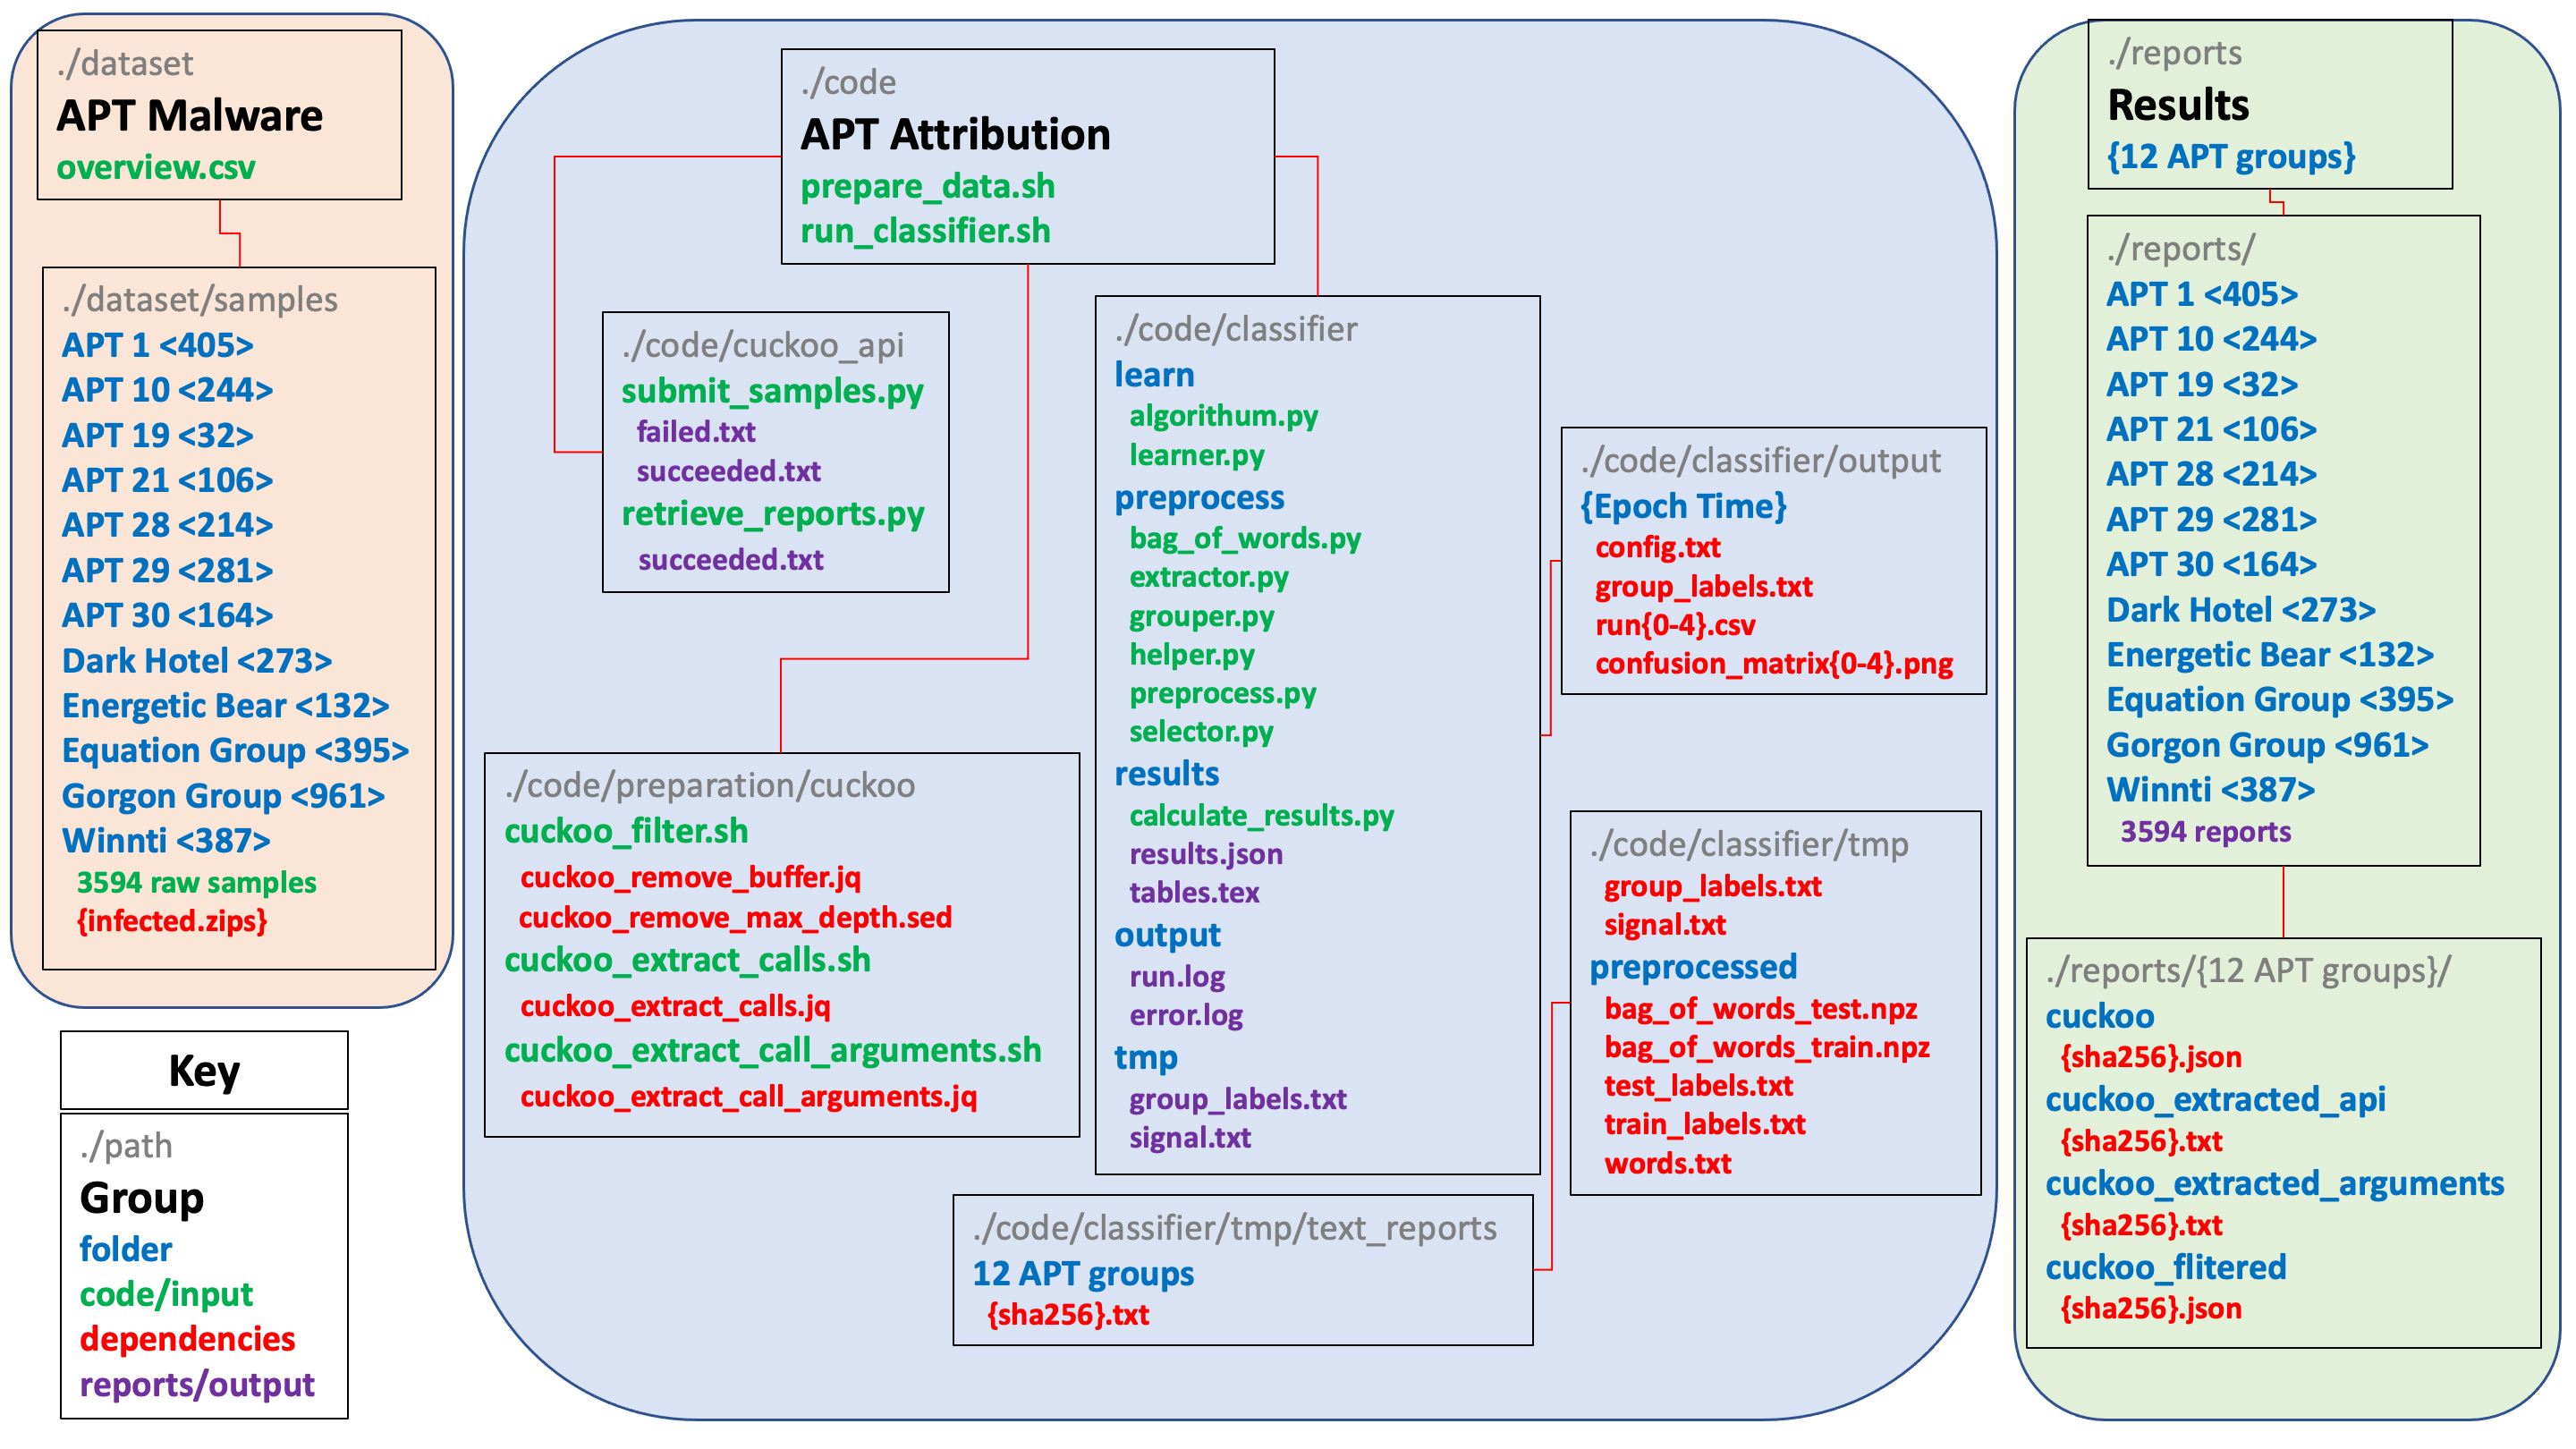
\includegraphics[width=1\textwidth]{images/APTAttribution-codebase.png}
	\caption{APTAttribution Codebase \protect\cite{APTAttribution2022}}
	\label{fig:APTAttribution-codebase}
\end{figure}

\begin{comment}
needed to allow analysis to be applied from multiple inputs across a timeline of events.  The Lockheed Martin Cyber Kill Chain allows analysis to take place at different stages with the natural cycle of a cyber attack without having to start from the beginning.  This is important because of the increased use of separate teams for areas of specialty that support the same mission.  Additionally, the state of digital security is such that most intermediate and advanced cyber threat actors are not found to have compromised a system for an extended period of time from when reconnaissance started.  There are the seven steps of the Cyber Kill Chain that describe the actions of a cyber threat: Reconnaissance, Weaponization, Delivery, Exploitation, Installation, Command and Control (C2), and Actions on Objectives \cite{martin2014cyber}.

``The MITRE ATT&CK knowledge base describes cyber adversary behavior and provides a common taxonomy for both offense and defense. It has become a useful tool across many cyber security disciplines to convey threat intelligence, perform testing through red teaming or adversary emulation, and improve network and system defenses against intrusions"  \cite{strom2018mitre}.   This framework can also be used to assist in the application of providence for the tactics and techniques to be define as adversarial behaviors within a lifecycle to a degree where they can be more effectively mapped to attribution.  The MITRE ATT&CK framework provides a granular view of the Delivery, Exploitation, Installation, C2 , and effects within the Cyber Kill Chain. 

The National Vulnerability Database (NVD) is a synchronized and searchable database of publicly disclosed cybersecurity vulnerabilities and exposures \cite{NIST_NVD:2020}.  The NVD consists of Common Vulnerabilities and Exposures (CVE) entries and is extended to include additional data such as fix information, severity scores, and impact ratings. As part of its enhanced information, NVD also provides advanced searching features such as by OS; by vendor name, product name, and/or version number; and by vulnerability type, severity, related exploit range, and impact.
\end{comment}

\section{Research Goals}
\begin{comment}
The primary goal of this research is to identify the minimum number of features that are required to maximize attribution and minimize computation.  Current capabilities within the area of identification of cyber threat actors (CTAs) based on their attack patterns extracted from cyber threat intelligence (CTI) reports using the distributional semantics technique of Natural Language Processing (NLP) show a precision rate of 83 percent \cite{noor2019machine}.  We aim to identify the computation efficient features in applying the accuracy of authorship attribution for malicious software samples. 
\end{comment}
The overarching goal of this research is to identify the minimum number of features required to attribute a malware sample to its author.  The objectives are 1) to reduce the noise inherent with a large feature set, 2) to increase accuracy, and 3) to reduce the computation resources required to perform authorship attribution.

\begin{comment}
DU comment on research goals "I don't know what this says" = 'map semantic data models in order to determine the linage of malicious software.'  Also, what does 'non-standard environments' "mean?"
	Map data models to apply?

What is the major contribution?  What is the CS link to changing the world?

20200722 - Pulled from first sentence of Research Goals "based on validated cyber threat intelligence and leverage the combined frameworks to enable forensic software analysis"
\end{comment}

\section{Research Plan}
\begin{comment} Look at integration into Ch.2...also need to reference Cuckoo sandbox
The novelty and utility of this research is to lessen the computational work needed to accurately apply cyber threat attribution.  Determining the role authorship plays in the similarity factor of software artifacts based on the providence of artifacts attributed to a specific threat actor enables analysis to react better when new threats emerge or change tactics.  In 2020, HP released a quarterly report on cyber threats that found "29\% of malware captured was previously unknown – due to the widespread use of packers and obfuscation techniques by attackers seeking to evade detection.  It took 8.8 days, on average, for threats to become known by hash to antivirus engines – giving hackers over a week’s ‘head-start’ to further their campaigns." \cite{HP-Bromium2020Q4report}  Research in applying computationally efficient attribution based on a particular software's attributes can be leveraged to react quicker to unknown threats.  If similar attributes are found in two or more different examples, then feature extraction can be used to describe their providence.  Computationally efficient feature extraction can also be applied over a large pool of malicious software examples in order to find trends in currently known capabilities and future focus areas.  The strength of this method for feature extraction is to increase the accuracy of applying cyber threat attribution with fewer resources.  In other words, the idea of applying augmented intelligence by using a novel approach to feature selection can increase the speed of applying cyber threat attribution.  
\end{comment}

\begin{comment}This research plan includes four parts: a dataset used an input, automated analysis platform, reporting infrastructure, and feature selection.  The dataset inputs will be structured in form of Advanced Persistent Threats (APT) that are separated by Country, APT Group, and Malware Family \cite{APTMalware2022}.  Table 3.1 gives a detailed overview of the contents of the APT Malware dataset used in this research.  It provides information on the raw malware samples collected from twelve identified Advanced Persistent Threats, their country of origin, malware family, and number of samples downloaded into the dataset.  
\end{comment}

We plan to conduct this research by first extracting features from a repository of malware samples that are attributed and  in common use by the cybersecurity research community, then selecting those features that provide the greatest accuracy for the least computational cost. 

\subsection{Feature Extraction}

The feature extraction phase consists of selecting the attributed malware dataset, profiling each artifact in the dataset through static and dynamic analysis, and identifying indicators of malicious action.     

Our background research uncovered three malware datasets that contain samples attributed to a specific author:   Laurenza \cite{laurenza2019daptaset}, cyber-research \cite{APTMalware2022}, and Haddadpajouh \cite{haddadpajouh2020mvfcc}.   The Laurenza dataset consists of 19 APT groups and over 2000 malware samples.  The cyber-research dataset contains 3594 malware samples which are related to twelve APT groups and five different nation-states.  The Haddadpajouh dataset consists of roughly 2000 samples and overlaps the cyber-research dataset.  We propose using the cyber-research dataset as it contains the largest number of attributed samples.    Table 3.1 overviews the cyber-research data with the number of malware samples attributed to APT Groups within respective countries. 

\begin{table}[h!]
  \scriptsize
  \centering
    \caption{APT Malware Dataset}
    \label{tab:table1}
    \begin{adjustbox}{width=\textwidth}
    \begin{tabular}{l|c|c|c|c} % <-- Alignments: 1st column left, 2nd middle and 3rd right, with vertical lines in between
      \textbf{Country} & \textbf{APT Group} & \textbf{Family} & \textbf{Sample Size}\\
      \hline
      China & APT 1 &  & 405 \\
      China & APT 10 & i.a. Plugx & 244 \\
      China & APT 19 & Derusbi & 32 \\
      China & APT 21 & TravNet & 106 \\
      Russia & APT 28 & *Bears* & 214 \\
      Russia & APT 29 & *Dukes* & 281 \\
      China & APT 30 & & 164 \\
      North-Korea & DarkHotel & DarkHotel & 273 \\
      Russia & Energetic Bear & Havex & 132 \\
      USA & Equation Group & Fannyworm & 395 \\
      Pakistan & Gorgon Group & Different RATs & 961 \\
      China & Winnti & & 387 \\
      \hline
      Total & & & 3594 \\
    \end{tabular}
  \end{center}
\end{table}

In researching malware analysis tools available that could be used to support the effort of preforming feature extraction of malicious samples, three products were investigated: Cuckoo, Remnux, and Bro.   Cuckoo  is a open source platform that automates malicious file analysis for Windows, OS X, Linux, and Android binaries.  Remnux is a Linux toolkit that assists analysts in reverse engineering malware samples.   Bro is a network-based analysis framework.  We propose using Cuckoo because it encompasses many of Remnux' and Bro's features, has an API that can be interfaced with for automation, and is open source.  

The software code base that controls the Cuckoo sandbox interacts in the following ways:  First, it manages the virtual machine image in which the malware is run.  Second, it executes each malware sample in the sandboxed virtual machine environment.  Third, it collects a variety of information from the sandbox, such as strings, PE sections, identification of packers, shell code, API calls, DLLs accessed, images of UI interaction, network connections, file manipulation, registry hives, and running processes.  Fourth, the analysis data is captured in JSON-formatted files.  Figure 3.1 provides a graphic description of the workflow as the dataset is ingested by the software code base to produce the reports. 

\begin{figure}
	\centering
	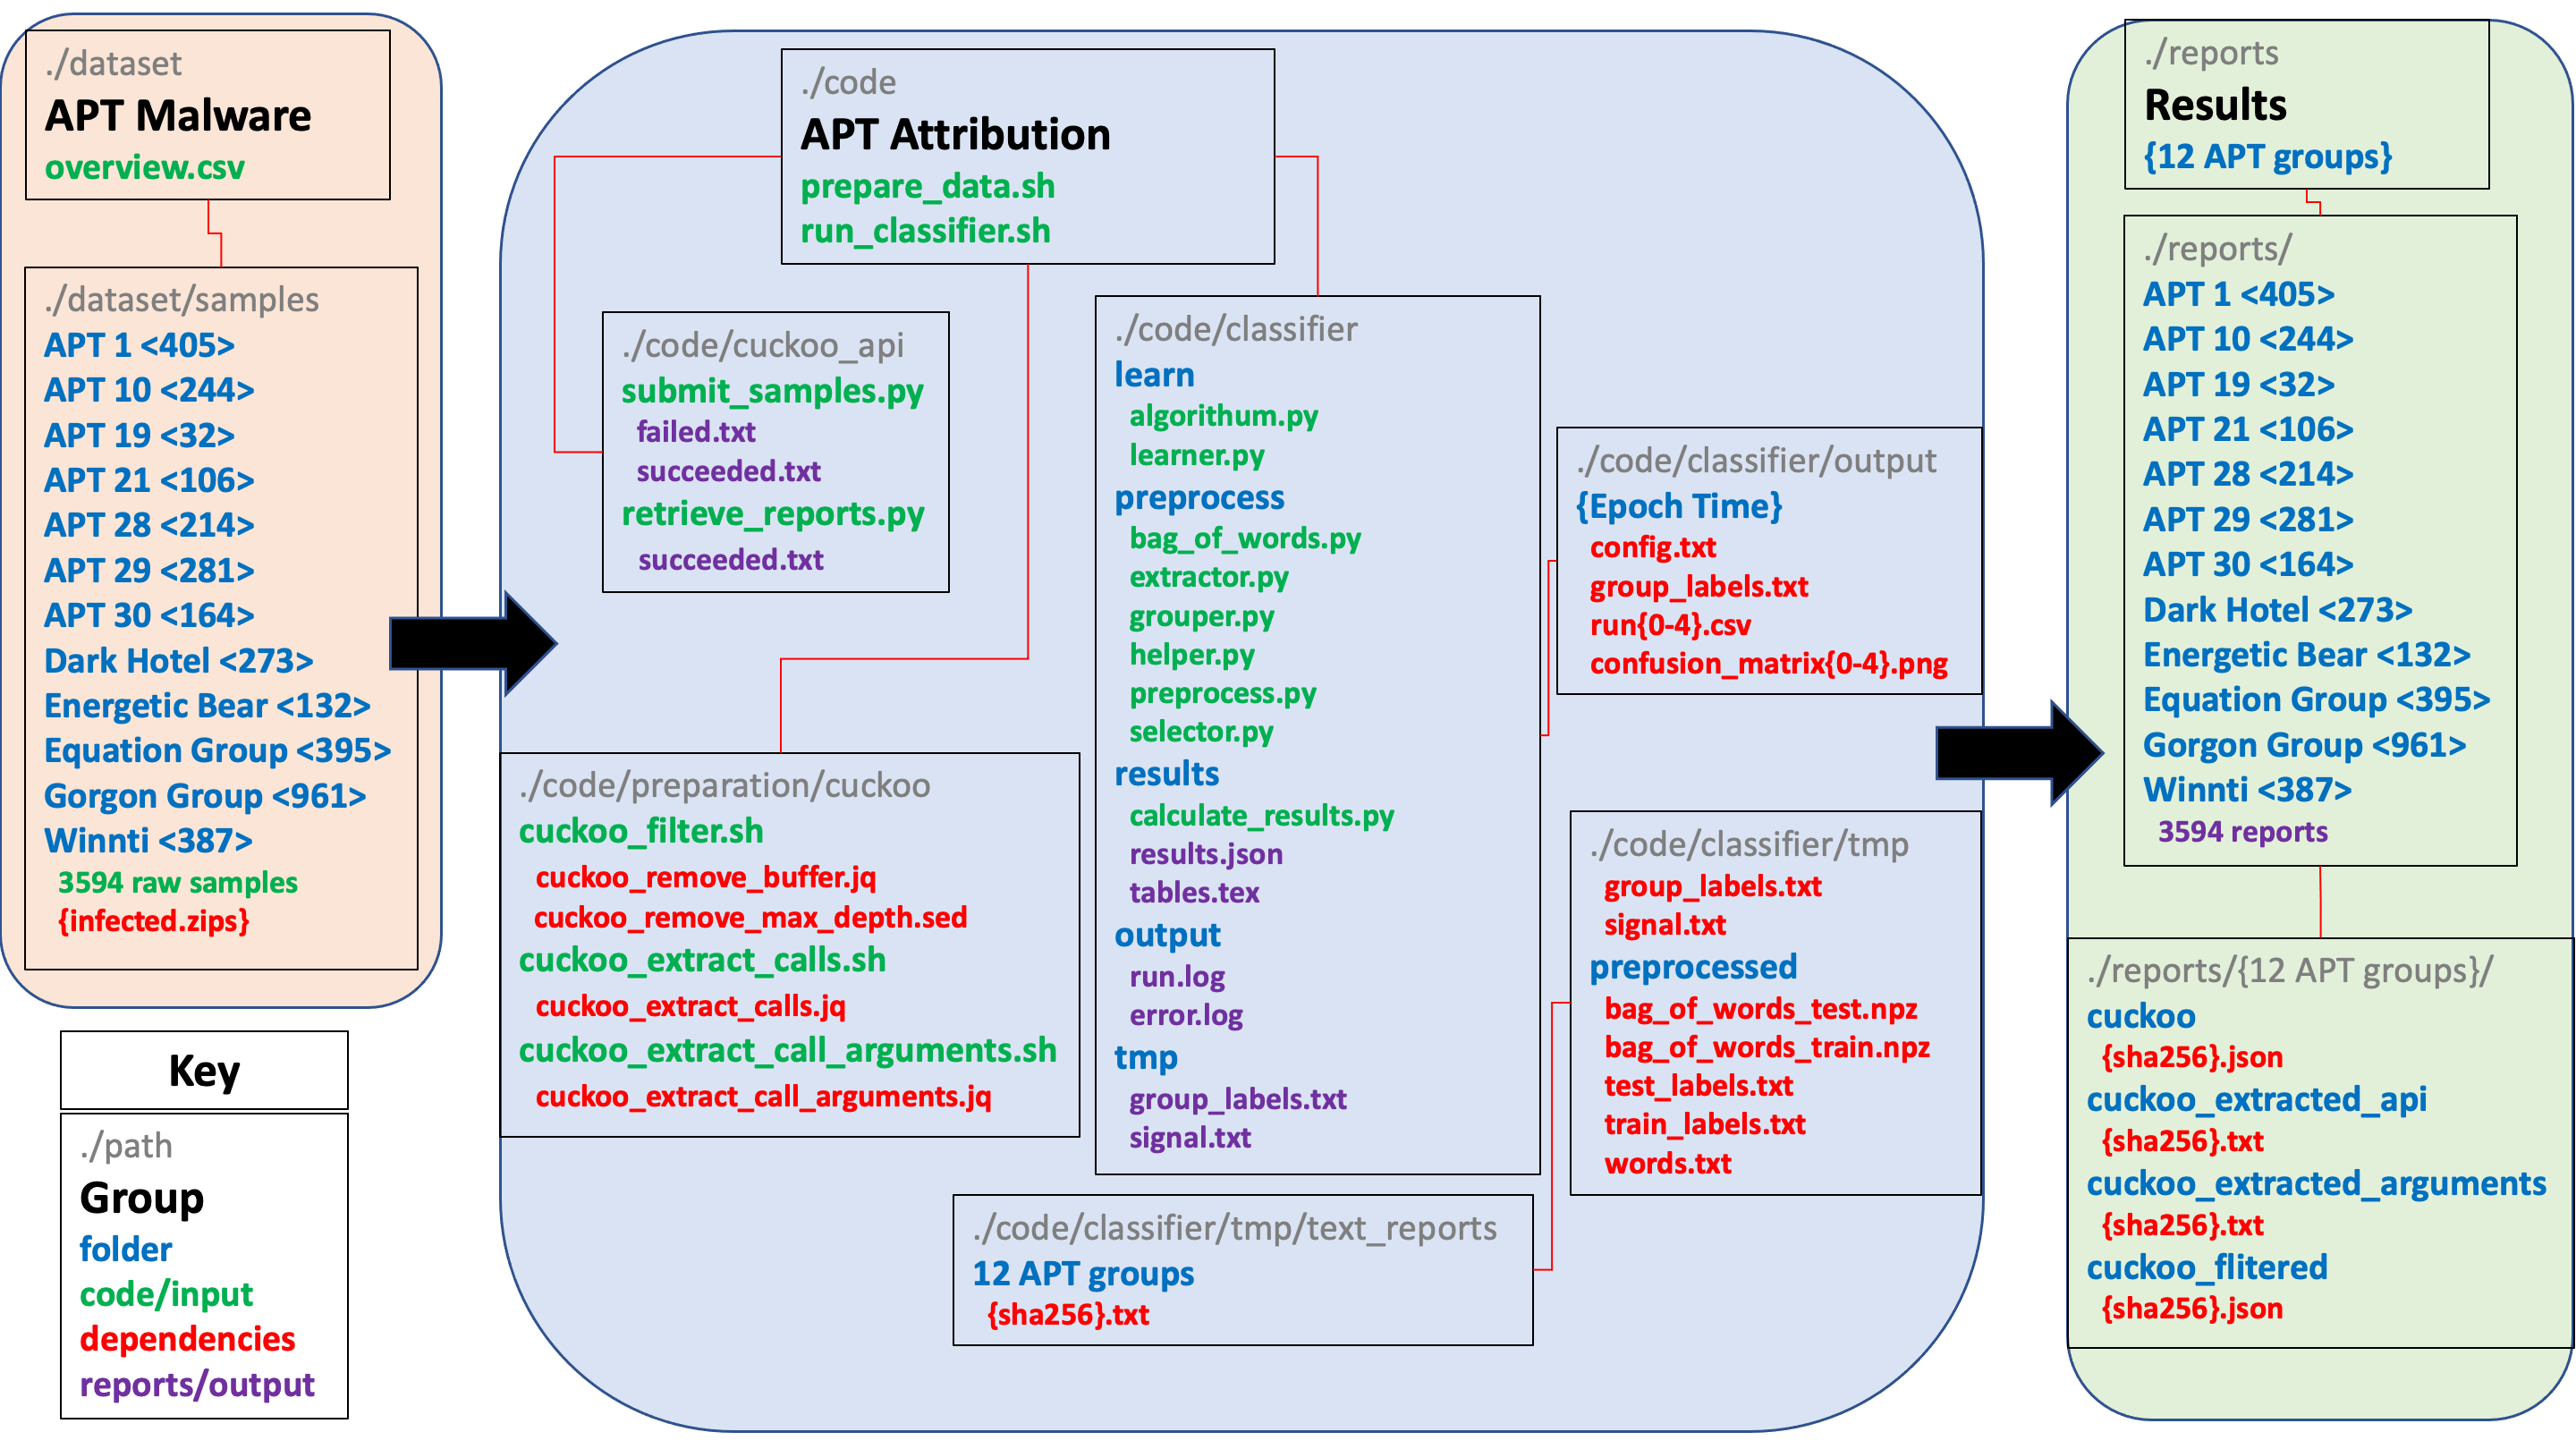
\includegraphics[width=1\textwidth]{images/APTAttribution-codebase-flow.png}
	\caption{Feature extraction workflow  \protect\cite{APTAttribution2022}}
	\label{fig:APTAttribution-codebase}
\end{figure}

In order to prepare the results to be analyzed, cleansing needs to be executed on the raw JSON report files for each sample.  The cleansing consists of two steps:  1) removing encrypted data that is specific to the malware instance but not generally useful to characterizing the malware sample and 2) extracting API calls and arguments.  Following the cleansing process, the json formatted reports are ready for feature pruning.  

\subsection{Feature Pruning}
The feature pruning phase identifies the most meaningful combinations of features required for attribution.  We propose doing this by using a combination of features identified by expert selection, then apply feature selection algorithm that improves attribution.

The identification and use of data modeling classification algorithms on the features will support data modeling classification as a structured method for validating the results.  Additionally, the aim is to also to promote future analysis by adding additional inputs into this modular framework.  In a comparison of data modeling techniques used in the research of applying attribution to threats the Random Forrest and Deep Neural Network Algorithms excelled \cite{gray2021identifying}.  Within the exploration of more than two classification algorithms, Random Forest (RF) was found to be the most suitable candidates for solving the problem due to their enhanced performance against the other techniques they tested  \cite{hong2018classifying}.  These results agree with additional research in the field: \cite{hendrikse2017effect}, \cite{caliskan2015coding}, \cite{kalgutkar2018android}, \cite{meng2016fine}, \cite{gonzalez2018authorship}.  The parameter values chosen for this data modeling classification algorithm is 100 estimators, meaning that 100 decision trees will run for this model.  Within the exploration other data modeling techniques, Deep Neural Network's showed usefulness for classifying binaries to authors better than Support Vector Machine (SVM) and Conditional Random Fields (CRFs): \cite{meng2018binary}, \cite{rosenberg2017deepapt}, \cite{rosenberg2018end}, \cite{alrabaee2019feasibility}, \cite{alrabaee2019bineye}.  The parameters values chosen for this data modeling classification algorithm is 7 layers of that range from 2000 to 500 nodes, that have a max of 250 iterations through which the data will be run.  These two data modeling classification algorithms show promise in assisting in this research.  Additionally, using more than one data modeling classification algorithm helps to fight potential bias present in the algorithms.

\begin{figure}
	\centering
	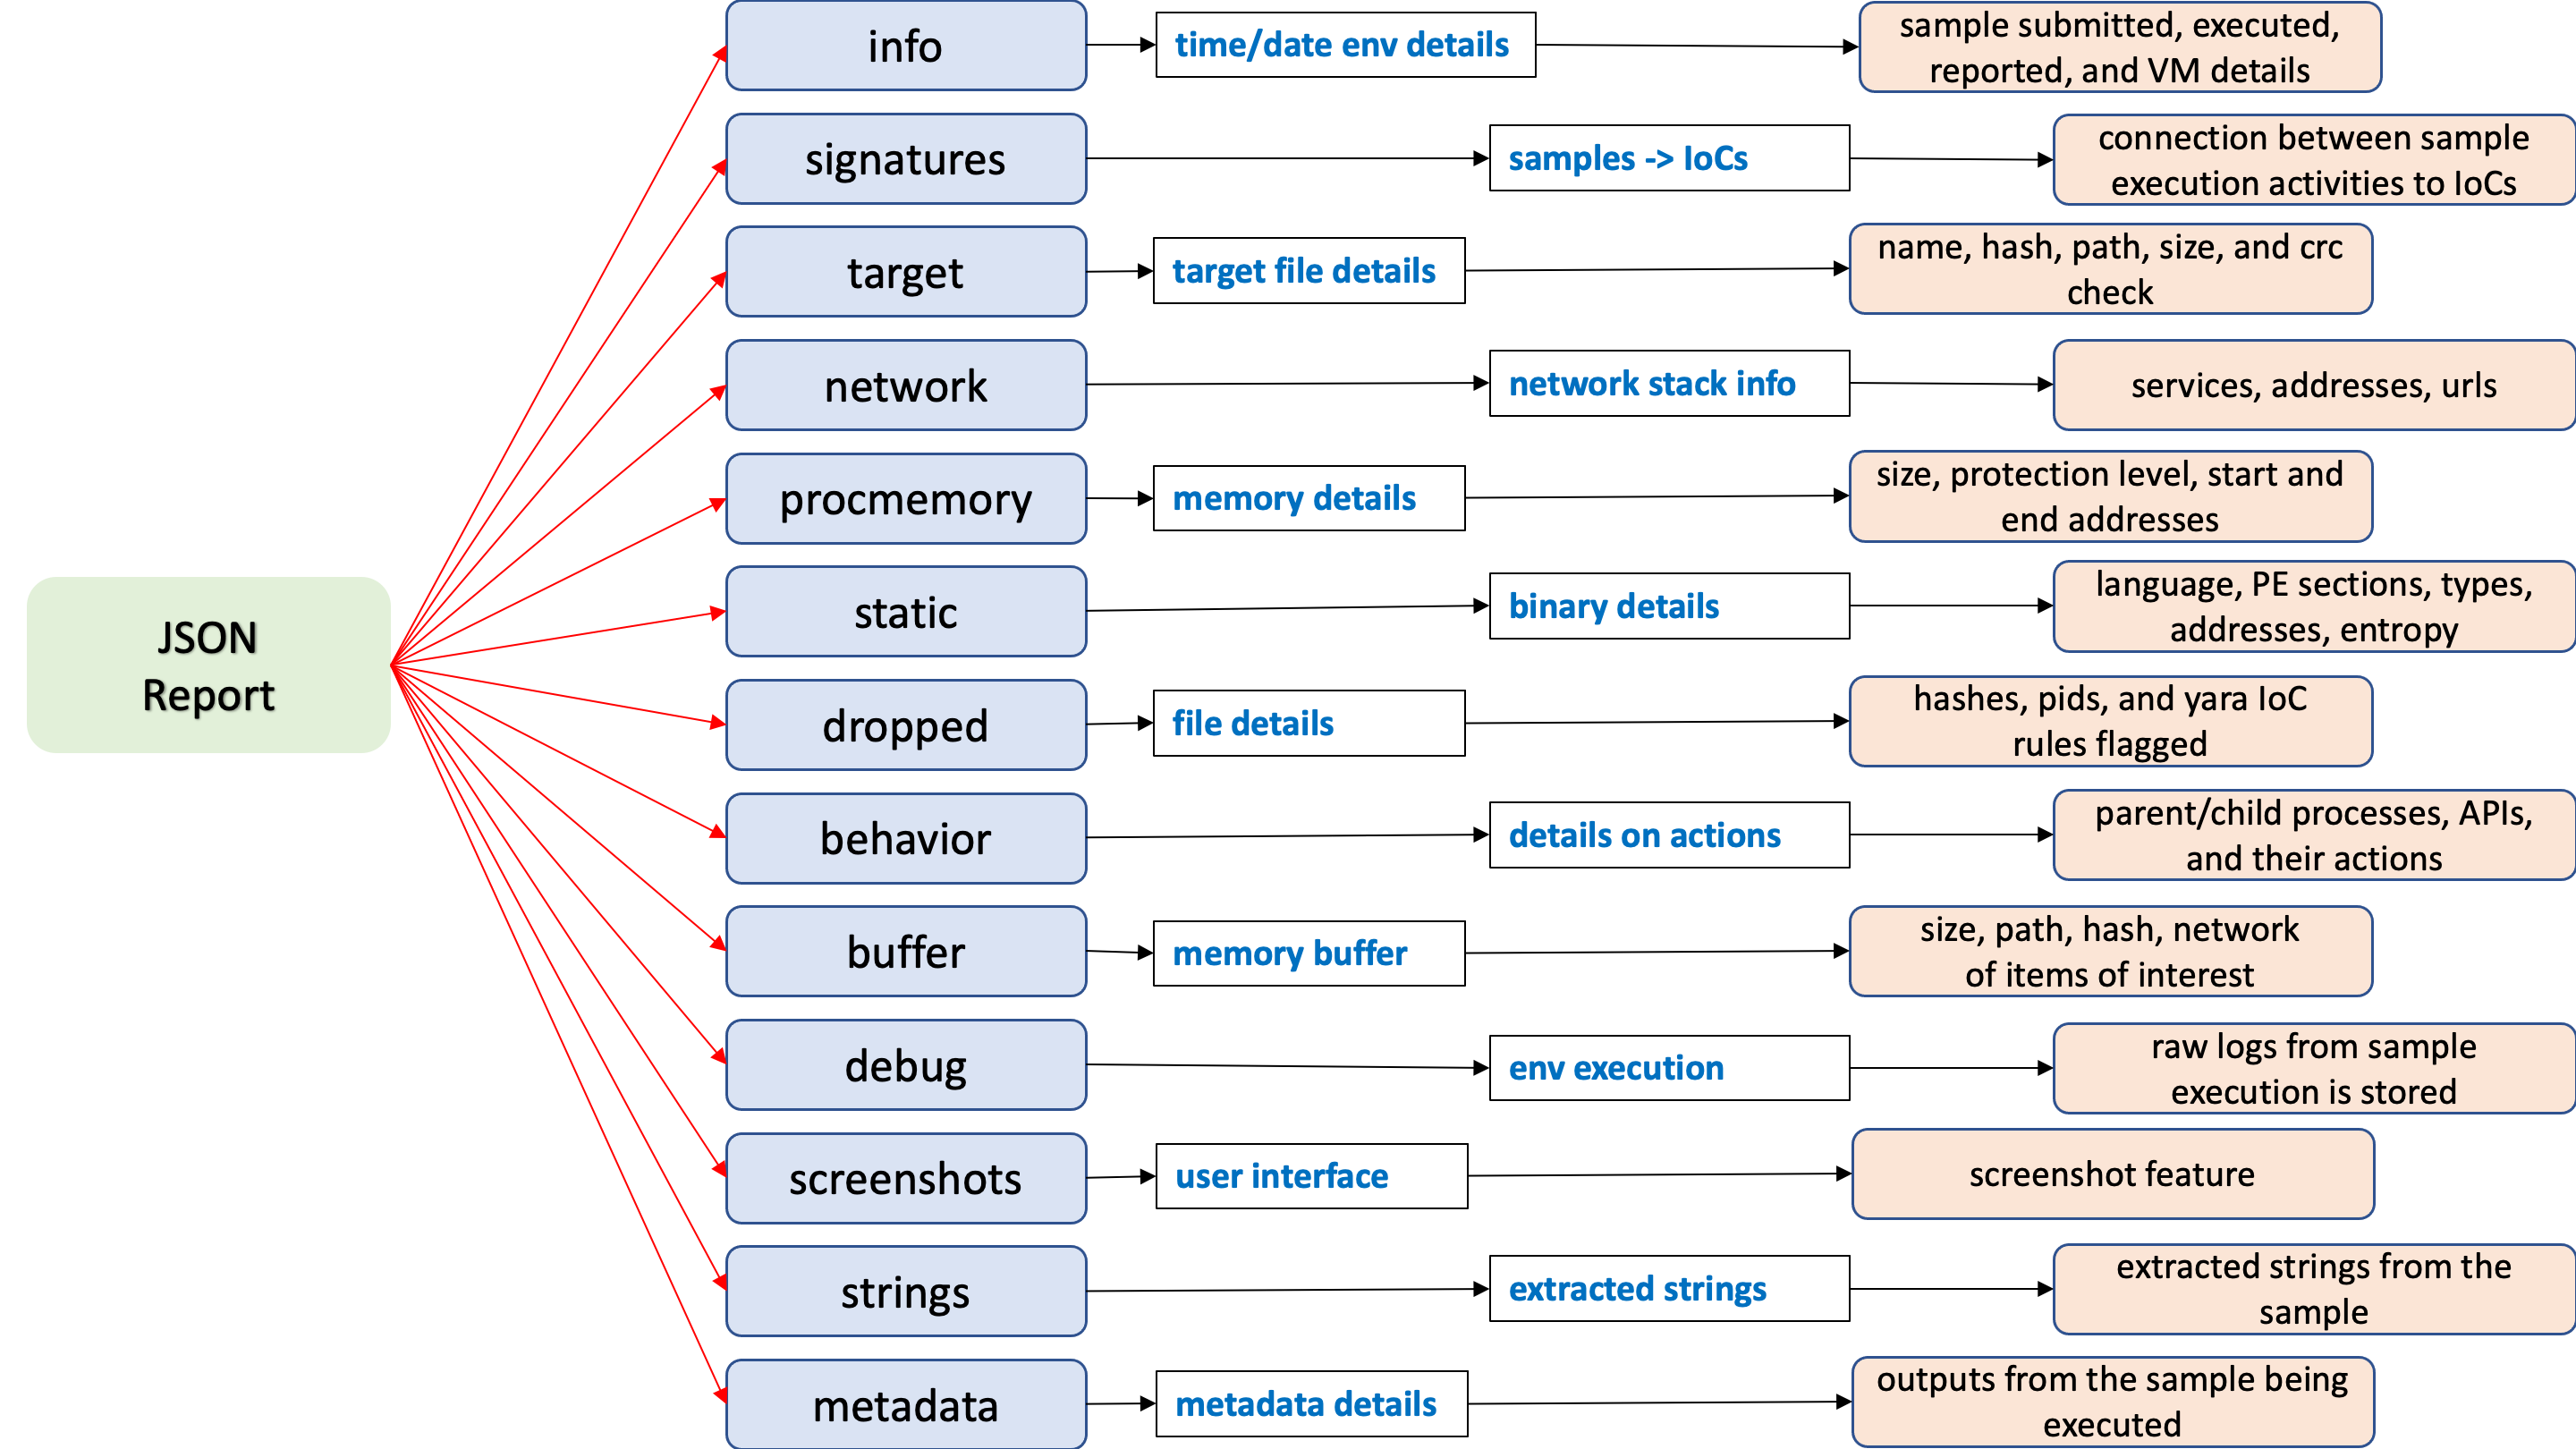
\includegraphics[width=1\textwidth]{images/JSON_Structure2.png}
	\caption{JSON Structure}
	\label{fig:JSON_Structure}
\end{figure}

Once the data modeling classification algorithms are selected they will be executed against all filtered and extracted results.  These results are collected that analyzed the accuracy of the classifiers correctly identifying the correct APT group when all features are present.  This give us a control state in which we can experiment using various combinations of feature selection. Then we will prune features in order to identify the best combination that provided a more efficient solution than currently recognized methods.  This method of data pruning is done though command line jq scripts on the .json formatted results.  An example of this pruning would be iterate over all json formatted results file to separate the data for the WriteProcessMemory API using this piped query string: .behavior.processes[].calls[] | select(.api == "WriteProcessMemory").api.    

\begin{figure}
	\centering
	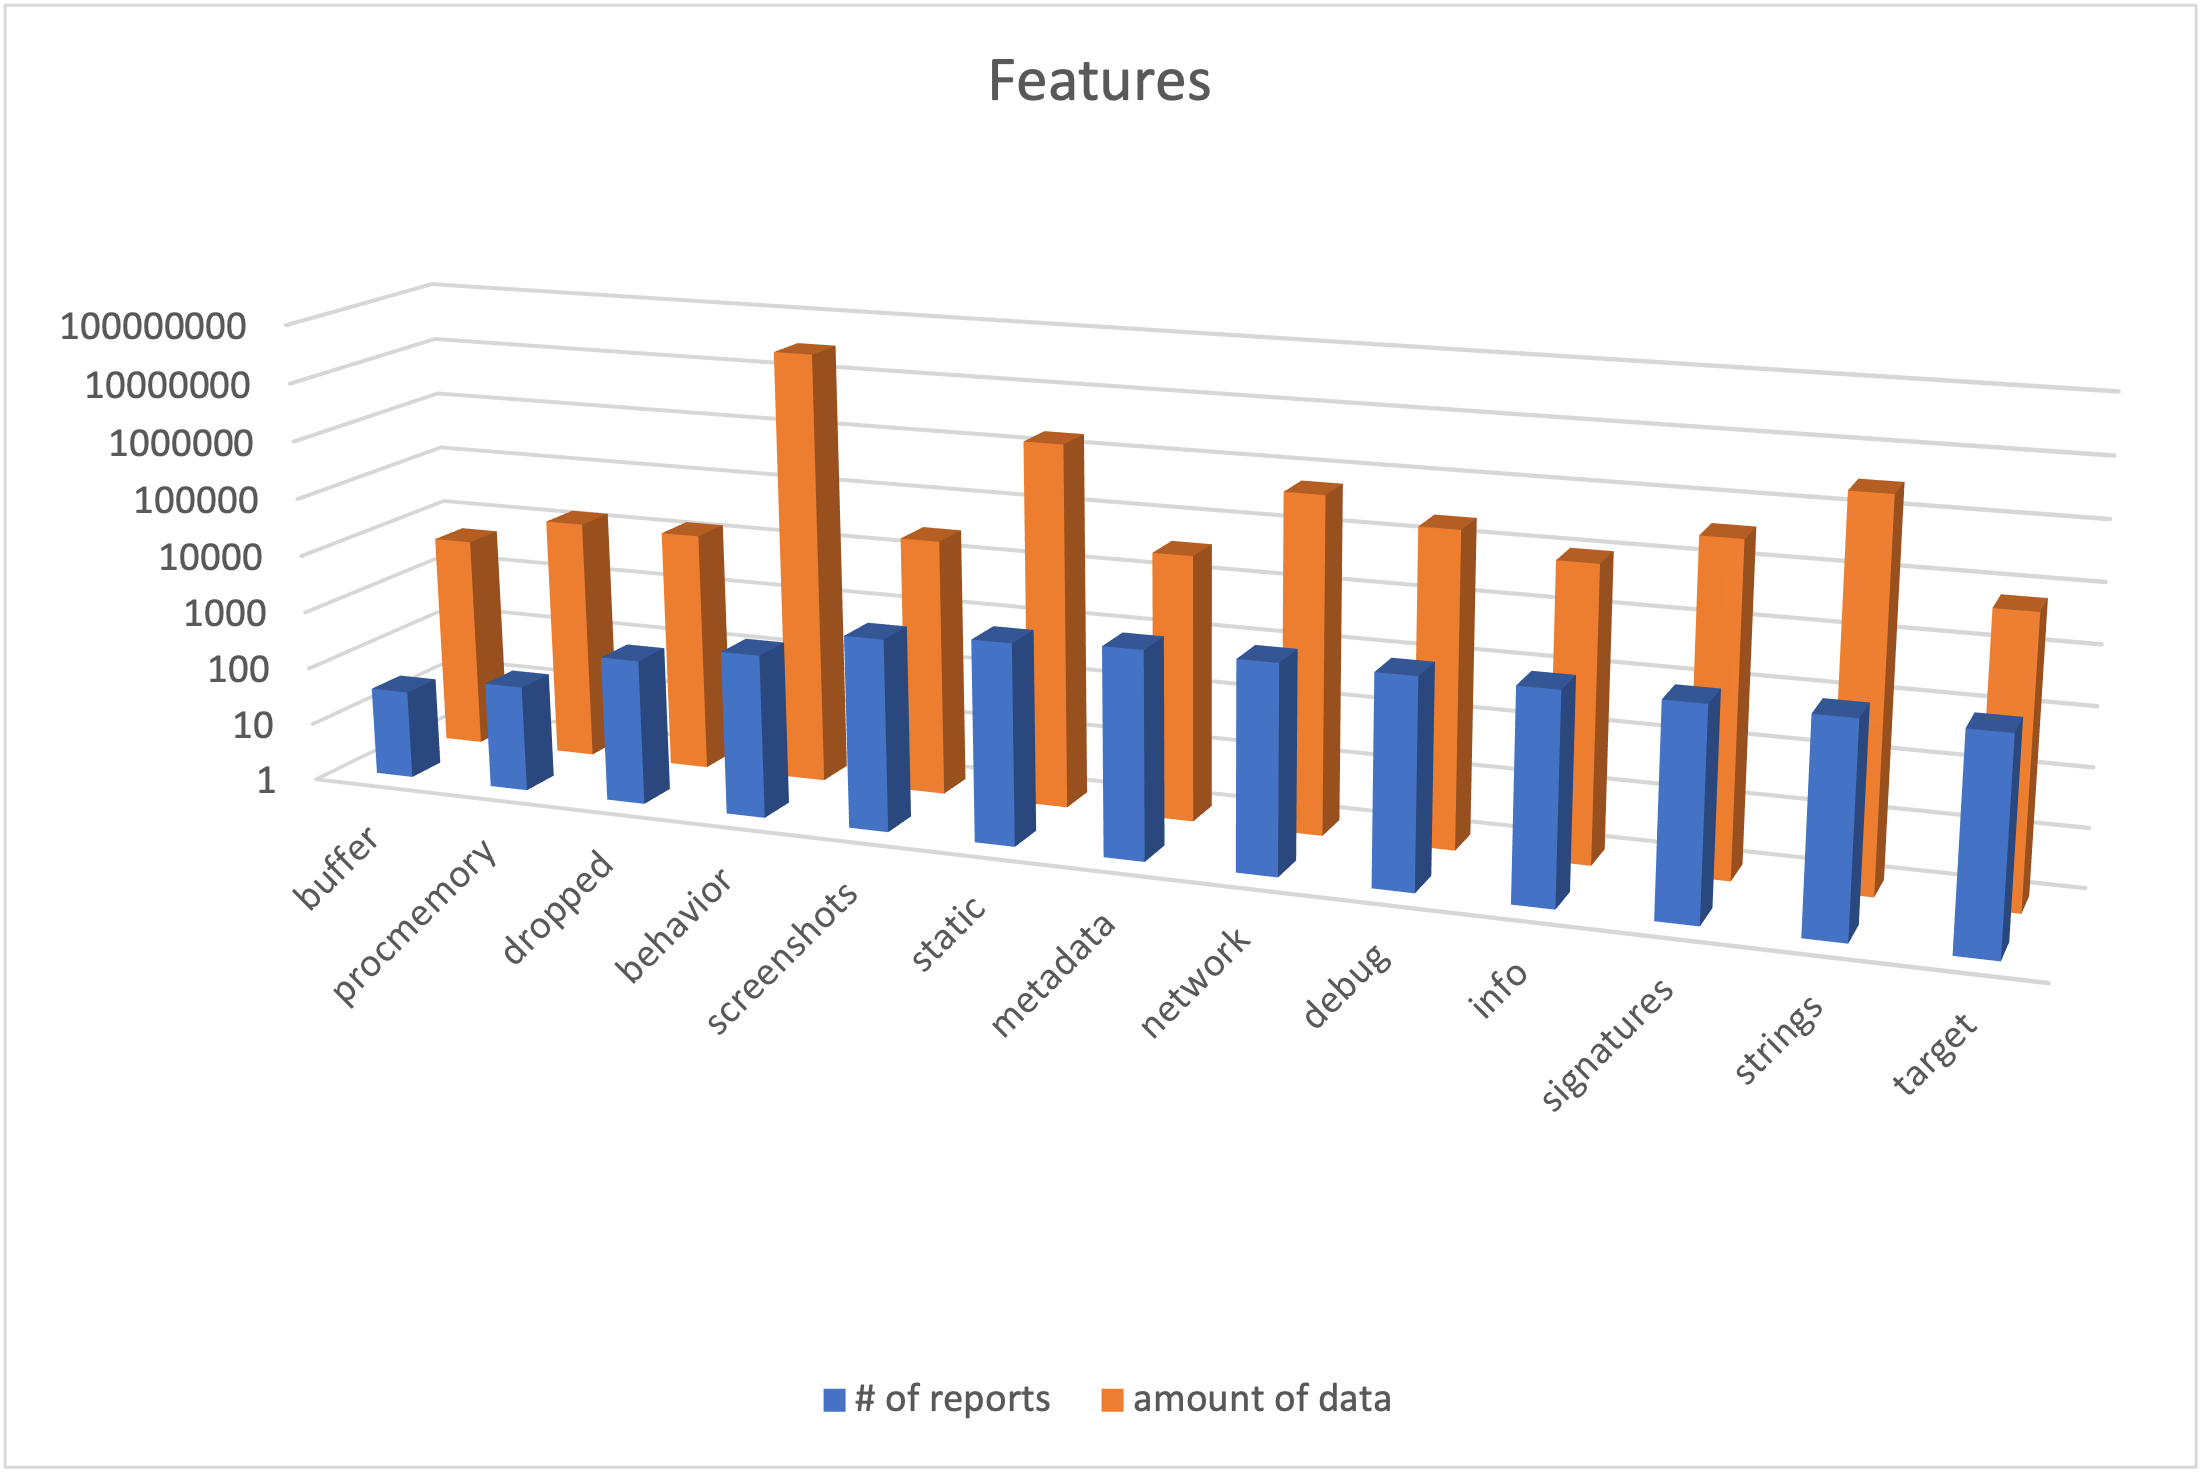
\includegraphics[width=.90\textwidth]{images/13_features_reports-vs-data.png}
	\caption{Features}
	\label{fig:Features}
\end{figure}

The ontology of these results is structured into 13 areas described in Figure 3.2.  The info feature contains information on the time/date that the sample submitted, executed, and reported on.  Also, it provides details on Virtual Machine that sample was run on.  Signatures provides a connection between sample execution activities to potential Indicators of Compromise (IoC).  The target group of features gives target file details, like: name, hash, path, size, and crc checks.  The collection of network information that emanated from the execution of the sample can be viewed in the network feature.  Procmemory shows the details about different regions of the memory with their size, protection level, start and end addresses.  The static feature displays information of the binary and its parts.  This information includes timestamp of when compiled, type of binary, resources used, language, PE sections, PE sections types, memory addresses, and level of entropy.  The dropped group of features provides information on dropped files, hashes, pids, and yara IoC rules flagged.  The behavior group collects information on parent/child processes, their relationships, APIs used, and their actions.  Information on the size, path, hash, network of items of interest in volatile memory is contained within the buffer group of features.  Debug is where raw logs from sample execution is stored.  Information about the user interface at different points during sample run can be referenced in the screenshot feature.  Strings contains extracted string from the sample.  Metadata includes information about various outputs from the sample being executed.  The scope of these json results include more than 38 million items, 1.35 million being unique, and an upper bound of 2.2 million instances.  The frequency of the total amount of reports and data point present in these reports for these thirteen different feature groups is displayed in Figure 3.3.

Expert selection will be used as the starting point of iteration of features in order to apply attribution.  This expert selection contains two steps, first step is to identify unique features that assist in attribution, second step is to eliminated duplicate data from the reports that will be given to the classifiers.  Based on the ontology of the data contained within the reports there are 6 different areas that expert selection points to in Cyber Threat Intelligence reports.  Two primary references are used in building this expert selection, the source column of the overview.csv file contained within the dataset selected for this research and additional supplemental reporting.  Most of the supplemental reporting has been collected from publicly-available papers and blogs of malicious campaigns/activity/software that have been associated with vendor-defined APT that are sorted by year and their source details stored on github. \cite{APTnotes}  

APT groups 19, 21, Gorgon, and Winnti all have uniquely identify items contained within the filepath area that support attribution based on expert opinion in CTI reporting \cite{DeepPanda2013}, \cite{ExploringBergard2016}, \cite{NewDerusbiFamily2015}, \cite{APT_Attacks2013}.  APT groups 1, 28, and 29 have information contained within function name arguments and strings that aid in applying attribution \cite{APT1Mandiant2013}, \cite{SofacyActivity2018}, \cite{DukeAPTcloudLin2015}.  APT 10 and the Energetic Bear groups are identifiable by looking for references to specific regkey read attempts \cite{OperationCloudHopperIoCs2017}, \cite{CrouchingYeti2014}.  Operations by APT 30 can be identified thought the use of mutant name argument \cite{APT30IoCs2015}.  The APT group known as Dark Hotel can be identified thought the used of a specific process name \cite{DarkHotelIoCs2014}.  Equation Group can be identified though the use of an identifiable string \cite{EquationSamples2015}.  The 6 areas for expert selection are using these combined sources are: function name, regkey read, filepath, mutant name, process name, and strings.

Iterations of different combinations of features will be generated in order to find the most effective way to apply attribution.  Confusion matrices generated from the data classification algorithms will be used to compare accuracy and drive the iteration process of identifying features that have the greatest rate of positive change for attribution accuracy.  The Proof of Concept section describes a specific scenario of feature pruning, analysis, and results.  Algorithm 1 is a pseudocode description of a novel methodology for combining Expert Selection with Genetic Algorithms (ESGA) for feature selection.

\begin{algorithm}
	\caption{Pseudocode of correlation-based ESGA method for feature selection}
	\begin{algorithmic}[1]
	\State \textbf{Input}{ F: feature, where feature = [data, velocity, dimension, weight]}  
	\State \textbf{Input}{ E: Let $E_{expert}$ = {e : F | human\_approved(e)}
	\State Extract keywords from $E_{expert}$
	\State { $E_0$ = Use keywords to filter F}

	\State { Let $E_{new}$ = deduplicate($E_0$)}

	\State \textbf{corr\_matrix}{ = corr(F,$E_{new}$)}
    	\State \textbf{Select}{ Select corr\_matrix.where(corr\_matrix.shape), k=1(bool)}
	
	\State \textbf{$E_{new}$}{ = Drop column for column in corr\_matrix.columns for any column $>$ 0.95}
	
	\State \textbf{$E_{old}$}{ = null}
	\While{notImproving($E_{old}$,$E_{new}$):}
	    \State \textbf{Repeat} {notImproving}{ $i=0$ \TO $3$ where population.accuracy -1\%}
		\State \textbf{Let}{ $confusionMatrix_1$ = classifier($E_{new}$)}
		\State \textbf{Let}{ $E_{changed}$ = geneticize($E_{new}$, F)}
	    \State \textbf{feature\_optimization\_matrix }{ = best population.accuracy(individual.X, individual.Y) from ($E_{new}$, F)}
			\State \textbf{Apply GA to k=1(feature)} 
			\State \textbf{Let $E_{changed}$}{ Select feature\_optimization\_martix.where(population.accuracy is greatest)} 
			
    	\State \textbf{Let}{ $confusionMatrix_2$ = classifier($E_{changed}$)}
    	\State \texbf{confusionMatrix = best($confusionMatrix_1$, $confusionMatrix_2$)}
    	\State \textbf{$E_{old}$}{ = $E_{new}$}
    	\State \textbf{$E_{new}$}{ = best($E_{new}$, $E_{changed}$)}
	\EndWhile

	\State \textbf{Output}{ $E_{new}$}
	\end{algorithmic} 
\end{algorithm}

The pseudocode in Algorithm 1 starts with the initialization of each individual data point in the feature collection.  Then the correlation coefficients between expert selected features and the contribution of each feature in all feature sets are calculated to obtain the improved initial value of the individual and the feature collection, as defined by lines 7 and 8.  The amount of correlation between these two parts is configured to 95\% similarity in this version of the algorithm.  The search process will stop and output the improved position of the feature collection, if the process comes to a stopping condition; otherwise, it will execute circularly.  The repeat conditions is defined based on control runs with all feature sets preset and configured to stop when the a decrease in accuracy exceeds the maximum allowable threshold.  This threshold is configured to be 3 consecutive instances of a greater than 1\% decrease in accuracy.  Lines 10–21 define the detailed cyclic process to get the improved feature subset, which contains updating the individual data points’ velocity and position, calculating the fitness value of the individual data point using classifiers, and updating the historical best position of the individual data point and the improved position of the feature collection.  The most improved feature subset will be selected after finishing this cyclical process.

\begin{comment}
***Expert Selection*** \\
spaCy - Industrial-Strength Natural Language Processing in Python
Prodigy - Radically efficient machine teaching.  An annotation tool powered by active learning.
More information: https://spacy.io and https://prodi.gy

***Genetic Algos*** \\
\end{comment}

\begin{comment}
The automated analysis platform used the open source malware analysis sandbox Cuckoo.  All 3594 samples were analyzed in this platform to enable feature set extraction of network, software, user, and other data inputs.  Samples were submitted and reports were returned to the reporting infrastructure though the use of cuckoo REST API.  The average run time for the submission, execution, and collection of the raw reports was around 200 hours.  

The reporting infrastructure is where the raw json formatted reports are housed.  These raw reports are formatted in two different ways in order to preform feature selection that can aid in authorship attribution.  First, the data is filtered in order to remove memory buffer information that does not aid authorship attribution and give the reports a consistent max depth.  Information related to the use of a packer and what level of entropy is present is collected before the memory buffer information is filtered.  Second, API calls and their arguments are extracted in order to provide feature set groupings between reported samples.

With the reports prepared we now analyze the results using two different classifiers with all available features present.  This includes all filtered and extracted data from the raw samples reports.  Results were collected that analyzed the accuracy of the classifiers correctly identifying the correct APT group when all features are present.  This give us a control state in which we can experiment using various combinations of feature selection. Then we will prune features in order to identify the best combination that provided a more efficient solution than currently recognized methods.

In the validation section we describe the process of comparing accuracy from all features to pruned features.  Samples with the combination of most frequent features extracted from the highest scoring malicious sample reports will be used in the initial validation process.  From there we will measure the accuracy of applying attribution from only using these extracted features.  Once accuracy is measured, the most efficient combination of features to apply attribution will be found using this framework.  In other words, the most frequent features will be extracted from the most malicious sample reports and accuracy will be measured from this starting point.  From this point going forward different combinations of feature sets will be used to identify an efficient solution to applying cyber threat attribution.  
\end{comment}

\begin{comment} look for a different reference that uses the same dataset...maybe https://www.hindawi.com/journals/scn/2021/8077220/#conclusions, references (Random Forests (RF) [50], [22], [54], [44] or Deep/Artificial Neural Networks (DNN/ANN) [103], [104], [78], [7], [8]) in https://arxiv.org/abs/2101.06124, or https://cs.ru.nl/~aserban/theses/b_coen_boot.pdf, and http://www.cs.ru.nl/E.Poll/papers/MalwareStateAttribution2019.pdf
This idea is similar to how \cite{oh2009fight} used variable-length fingerprints across a series of instructions to describe how data is used within a function or basic block.  The order and path of data transformations are important and uniquely identifiable, such as in the same way that an mystery author's work can be identified because of key characteristics.  Key characteristics in analyzing the most frequent features extracted from the highest scoring malicious samples are: APIs called, arguments given, PE section details, entropy measurement, and file details.
\end{comment}

\begin{comment}
A focus has been made to standardized formats of Cyber Threat Information (CTI) in order to increase data sharing.  The Malware Information Sharing Platform (MISP) is an open source platform that can be used for gathering, sharing, storing, and correlating a number of structured and unstructured inputs about cyber threats \cite{MISP}.  Examples of common MISP feeds are Indicators of Compromise of targeted attacks, threat intelligence, financial fraud information, and vulnerability information.  We will use the MISP platform for collection and analysis of inputs of authorship attribution based on levels of confidence.  Data from this platform will be used to create training data for an augmented intelligence system that leverages Natural Language Processing.

DU comments on last paraphgraph within 'Research Idea' = "while this is a good 100k-foot descroption, we need a more deailed explanation"

	DU = Change reference display from '[Oh 2009]' to "Oh [2009]"
	
20200722 - Open Standards For Threat Information Sharing
\end{comment}

\section{Proof of Concept}
The sandboxed virtual machine environment is comprised of a Intel i9 CPU fitted into a Socket LGA 2066 motherboard with 32 GigaBytes of DDR4 RAM.  The RAM is configured to run at a speed of 3600 Megahertz.  Two EVGA GeForce GTX 1080 Ti FTW3 HYBRID cooled GPUs are connected together using an SLI bridge to provide video output and computational support using cuda.  Additionally, two 250 GigaByte Samasung 850 Pro Solid State Drives connected in a RAID 0 are formated for the boot partition and storage of the raw results.  To illustrate the feasibility of our approach, we implemented Algorithm 1 on a limited subset of data.  We started by ingesting the cyber-research [Radnus 2022b] dataset into the Cuckoo Sandbox software tool.  The tool required roughly 700 hours to analyze the 3594 samples of the dataset and produce the raw results described in Figure \ref{fig:JSON_Structure}.  We applied two classification algorithms – Random Forrest Classifier (RFC) and Deep Neural Net (DNN) classifier -- to the raw results to establish an analysis baseline that takes into consideration the entire dataset.  We also applied the classifier algorithms to a subset of the raw results so as to demonstrate how to select and measure combinations of features that might reduce the noise of the entire data set and lead to better performance.  We refer to the former analysis as the “control results” and the latter analysis as the “extracted results.”

Table 3.2 shows the accuracy of control results obtained from the RFC and DNN classification algorithms.  These control results are used to describe the accuracy of applying attribution using all available features from the dataset results.  These results include features from static/dynamic software analysis, volatile memory, and network actions.  These features are used by the classifiers to apply attribution across the twelve identified Advanced Persistent Threats in table 3.1.  There are 3 specific group comparisons that are preformed in this analysis.  The first, APTGrouper is focused on grouping attributed samples from specific APTs.  The second is focused on grouping attributed samples from specific countries.  The third is a combination of countries separated along with grouping based on the malware family.  Both RFC and DNN are applied to each of these groupers to measure the accuracy of applying attribution within these groups.  The Dataset column describes the source of the results.  Within the Dataset column, the ``Cuckoo" label designates all filtered results were used and ``Cuckoo*" designates the pruned results were used.  The next three columns represent accuracy results and the standard deviation of those results described in the form of a lowercase Sigma.  In order to adjust for bias within the Groupers Unbalanced, Undersampling, and Oversampling accuracy are recorded and displayed.  The problem of having imperfect or unbalanced data will always be present, but can be measured to provide guidance in the correct direction.  For the chosen dataset there is a clear imbalance between the Country Group China having 1338 samples out of the 3594 total samples in table 3.1.  These results amount to around 37\% of the total samples within the five different Countries of this group.  This matters because building a classifier using the data as it is, would in most cases give us a prediction model that is always biased towards the Chine Country Group class.  The classifier used would be biased without preprocessing.  There are three things to do when dealing with imbalanced data:
% Create Nested unordered lists in LaTeX
\begin{itemize}
  \item Ignoring the problem.
    \begin{itemize}
    \item Building a classifier using the data as it is, would in most cases give us a prediction model that always returns the majority class. The classifier would be biased and the world is not a better place.
  \end{itemize}
  \item Undersampling the majority class.
  \begin{itemize}
    \item One of the most common and simplest strategies to handle imbalanced data is to undersample the majority class.  While different techniques have been proposed in the past, typically using more advanced methods (e.g. undersampling specific samples, for examples the ones “further away from the decision boundary”) \cite{japkowicz2000class} did not bring any improvement with respect to simply selecting samples at random.  For this analysis we selected n samples at random from the majority class, where n is the number of samples for the minority class, and use them during training phase.  These samples will be excluded for use in validation.
  \end{itemize}
    \item Oversampling the minority class.
  \begin{itemize}
    \item Oversampling the minority class can result in overfitting problems if we oversample before cross-validating.  A currently well recognized method for this is the Synthetic Minority Oversampling Technique (SMOTE) technique \cite{chawla2002smote}.  SMOTE is a method that instead of simply duplicating entries creates entries that are interpolations of the minority class, as well as under samples the majority class. Normally when we duplicate data points the classifiers get very convinced about a specific data point with small boundaries around it, as the only point where the minority class is valid, instead of generalizing from it.  SMOTE however effectively forces the decision region of the minority class to become more general, partially solving the generalization problem.  In simplest terms, oversampling using SMOTE improves the decision boundaries in imbalanced data.
  \end{itemize}
\end{itemize}

Multiple controls runs were executed and results were within 1.5\% accuracy and 0.02 standard deviation.

\begin{table}[h!]
    \centering
        \caption{Control Results}
        \label{tab:table2}
        \begin{width=\textwidth}

        \begin{tabular}{l|l|r|r|r}
            \multicolumn{5}{l}{APTGrouper} \\
                     & \textbf{Dataset} & \textbf{Unbalanced} & \textbf{Undersampling} & \textbf{Oversampling} \\ \hline
            \multirow{RFC} & Cuckoo & 0.40 ($\sigma$: 0.01) & 0.17 ($\sigma$: 0.03) & 0.22 ($\sigma$: 0.02) \\
            \multirow{DNN} & Cuckoo & 0.40 ($\sigma$: 0.01) & 0.13 ($\sigma$: 0.07) & 0.21 ($\sigma$: 0.03) \\
        \end{tabular}


        \begin{tabular}{l|l|r|r|r}
            \multicolumn{5}{l}{CountryGrouper} \\
                     & \textbf{Dataset} & \textbf{Unbalanced} & \textbf{Undersampling} & \textbf{Oversampling} \\ \hline
            \multirow{RFC} & Cuckoo & 0.44 ($\sigma$: 0.01) & 0.28 ($\sigma$: 0.01) & 0.28 ($\sigma$: 0.01) \\
            \multirow{DNN} & Cuckoo & 0.44 ($\sigma$: 0.00) & 0.27 ($\sigma$: 0.01) & 0.28 ($\sigma$: 0.01) \\
        \end{tabular}


        \begin{tabular}{l|l|r|r|r}
            \multicolumn{5}{l}{CountrySeparatedGroupAndFamiliesGrouper} \\
                     & \textbf{Dataset} & \textbf{Unbalanced} & \textbf{Undersampling} & \textbf{Oversampling} \\ \hline
            \multirow{RFC} & Cuckoo & 0.67 ($\sigma$: 0.01) & 0.35 ($\sigma$: 0.01) & 0.34 ($\sigma$: 0.01) \\
            \multirow{DNN} & Cuckoo & 0.67 ($\sigma$: 0.01) & 0.34 ($\sigma$: 0.02) & 0.33 ($\sigma$: 0.01) \\
        \end{tabular}
    \end{center}
\end{table}

The second part of the proof of concept was the application of feature pruning using expert selection.  Expert selection was preformed on the collected control results of the most maliciously scored samples collected.  There were a total of 17 malware sample reports that fell into the highest threat level range of 7-10 and were categorized as very malicious.  Within these 17 high scoring results, 5 distinguishing types of feature sets were contained within these samples.  These feature sets are categorized as: APIs, arguments, PE sections, entropy, and file details.  In total, there were 167 API calls in the 17 samples that were captured.  There were 17 instances of the API WriteProcessMemory being used in reports for this threat level.  Data pruning was executed to isolate on the API WriteProcessMemory calls and associated API arguments from this round of classification.

Table 3.3 describes the pruned analysis results that show the rate of change in attribution based on two changes to the API WriteProcessMemory pruned results.  The accuracy and standard deviation calculations in red have shown the change in applying attribution using only the API WriteProcessMemory calls and associated API arguments.  

\begin{table}[h!]
    \centering
        \caption{API WriteProcessMemory Extracted Results}
        \label{tab:table2}
        \begin{width=\textwidth}

        \begin{tabular}{l|l|r|r|r}
            \multicolumn{5}{l}{APTGrouper} \\
                     & \textbf{Dataset} & \textbf{Unbalanced} & \textbf{Undersampling} & \textbf{Oversampling} \\ \hline
            \multirow{RFC} & Cuckoo* & 0.28 ($\sigma$: 0.01) & 0.16 ($\sigma$: 0.09) & 0.05 ($\sigma$: 0.01) \\
            \multirow{DNN} & Cuckoo* & 0.27 ($\sigma$: 0.00) & 0.07 ($\sigma$: 0.00) & 0.08 ($\sigma$: 0.03) \\
        \end{tabular}

        \begin{tabular}{l|l|r|r|r}
            \multicolumn{5}{l}{CountryGrouper} \\
                     & \textbf{Dataset} & \textbf{Unbalanced} & \textbf{Undersampling} & \textbf{Oversampling} \\ \hline
            \multirow{RFC} & Cuckoo* & 0.38 ($\sigma$: 0.00) & 0.17 ($\sigma$: 0.06) & 0.15 ($\sigma$: 0.03) \\
            \multirow{DNN} & Cuckoo* & 0.37 ($\sigma$: 0.00) & 0.21 ($\sigma$: 0.10) & 0.17 ($\sigma$: 0.03) \\
        \end{tabular}

        \begin{tabular}{l|l|r|r|r}
            \multicolumn{5}{l}{CountrySeparatedGroupAndFamiliesGrouper} \\
                     & \textbf{Dataset} & \textbf{Unbalanced} & \textbf{Undersampling} & \textbf{Oversampling} \\ \hline
            \multirow{RFC} & Cuckoo* & \colorbox{green}{0.70} ($\sigma$: 0.00) & 0.30 ($\sigma$: 0.00) & 0.30 ($\sigma$: 0.00) \\
            \multirow{DNN} & Cuckoo* & \colorbox{green}{0.70} ($\sigma$: 0.00) & 0.38 ($\sigma$: 0.16) & 0.46 ($\sigma$: 0.19) \\
        \end{tabular}
    \end{center}
\end{table}

The accuracy results from the API WriteProcessMemory Extracted Results show an increase in accuracy for the unbalanced measurement of the Country Separated Group And Families Grouper highlighted in green.  Additionally, there are significant changes in accuracy results for the both classifiers executed in the APTGrouper and CountryGrouper runs.  The average rate of change between the positive accuracy of the Control and API WriteProcessMemory Extracted Results with both classifiers are within 8-11\% for the APT and Country Groupers.  Significant change was also observed in standard deviation within the extracted results for Undersampling in all groups, except for Random Forrest in the Country Separated Group And Families Grouper.  Additionally, the largest difference in standard deviation was found in Oversampling of the Deep Neural Network Classification in the Country Separated Group And Families Grouper.  These results lead to the conclusion that the API WriteProcessMemory features have a strong connection to apply attribution within this dataset, especially in the Country Separated Group And Families Grouper.  The research plan section describes the plan to extending this research in order to show the efficiency of applying attribution using expert selection on additional extracted data input.  Measurements within these results of accuracy between the control and pruned results will be the validation mechanism for this research.

\section{Research Hypothesis} 
The research hypothesis is ``the expert selection correlation mapping technique of feature selection using genetic algorithms is be more efficient than current recognized methods in applying cyber threat attribution''. The null hypothesis of this research is ``the expert selection correlation mapping technique of feature selection using genetic algorithms is as efficient or less efficient than current recognized methods in applying cyber threat attribution''.  More and less efficient is defined as recent applications of technology in the realm of authorship attribution methods that have an accuracy of 88\%.

\begin{comment}

DU "think of a hypothesis as being a metric by which you will know when you are done.  Consider phrasing the hypothesis in measuable terms.  Also section 3.2 suggests you have two hypothesises"

	Change your research hypothisis
		state your requirement as a yes or no
		what signture based techniquences

		research plan - current validation section Pytorch and Tensor Flow
		null hypothsis - will not preform any better than the current state of the art
\end{comment}  

\section{Research Plan}
Using the same dataset, results, and software code base the research will follow the same path a described in the proof of concept section.  A control run of random features will be used to create the control results for comparison.  Then features identified by expert selection will be chosen by using cyber threat intelligence reports for APTs in the chosen dataset.  Key words, phrases, and numbers will be picked from the reports to be used in selecting features.  Second, data de-duplication will be done between the features selected and additional features available from the dataset reports.  A comparison function will be used to find duplicate data that is similar within the data in selected features.  A configurable variable of 95\% is planned to be used as the starting point of this research, but can be modified to meet the needs of other research efforts.  The reason for this is to reduce unneeded duplication of data that will not assist with the task of accuracy of authorship attribution.  The third part is the initialization and recurrence of measurements for cyber threat attribution accuracy based on a genetic algorithm being applied to the de-duplicated data.  The genetic algorithms that are planned for comparison and correlation of expert selection are: Genetic \& Evolutionary Feature Selection (GEFeS), Particle Swarm Optimization (PSO), Artificial Bee Colony Optimization (ABCO), Ant System Optimization (ASO), and Glowworm Swarm Optimization (GSO).  In the same way that accuracy was measured in the proof of concept, accuracy and standard deviation will be the primary measurements of the research.

A configurable repeat until clause stop the recursion based on measurements gain from multiple control runs on all features being available.  For this research this clause is configured to trigger when 3 consecutive runs happen in which a -1\% accuracy is observed though the application of the genetic algorithm.  The last part is the building and reporting of a confusion matrix in order to graphically display the results to humans and allow for further research to be developed and tested. 

\begin{comment}

\begin{figure}
	\centering
	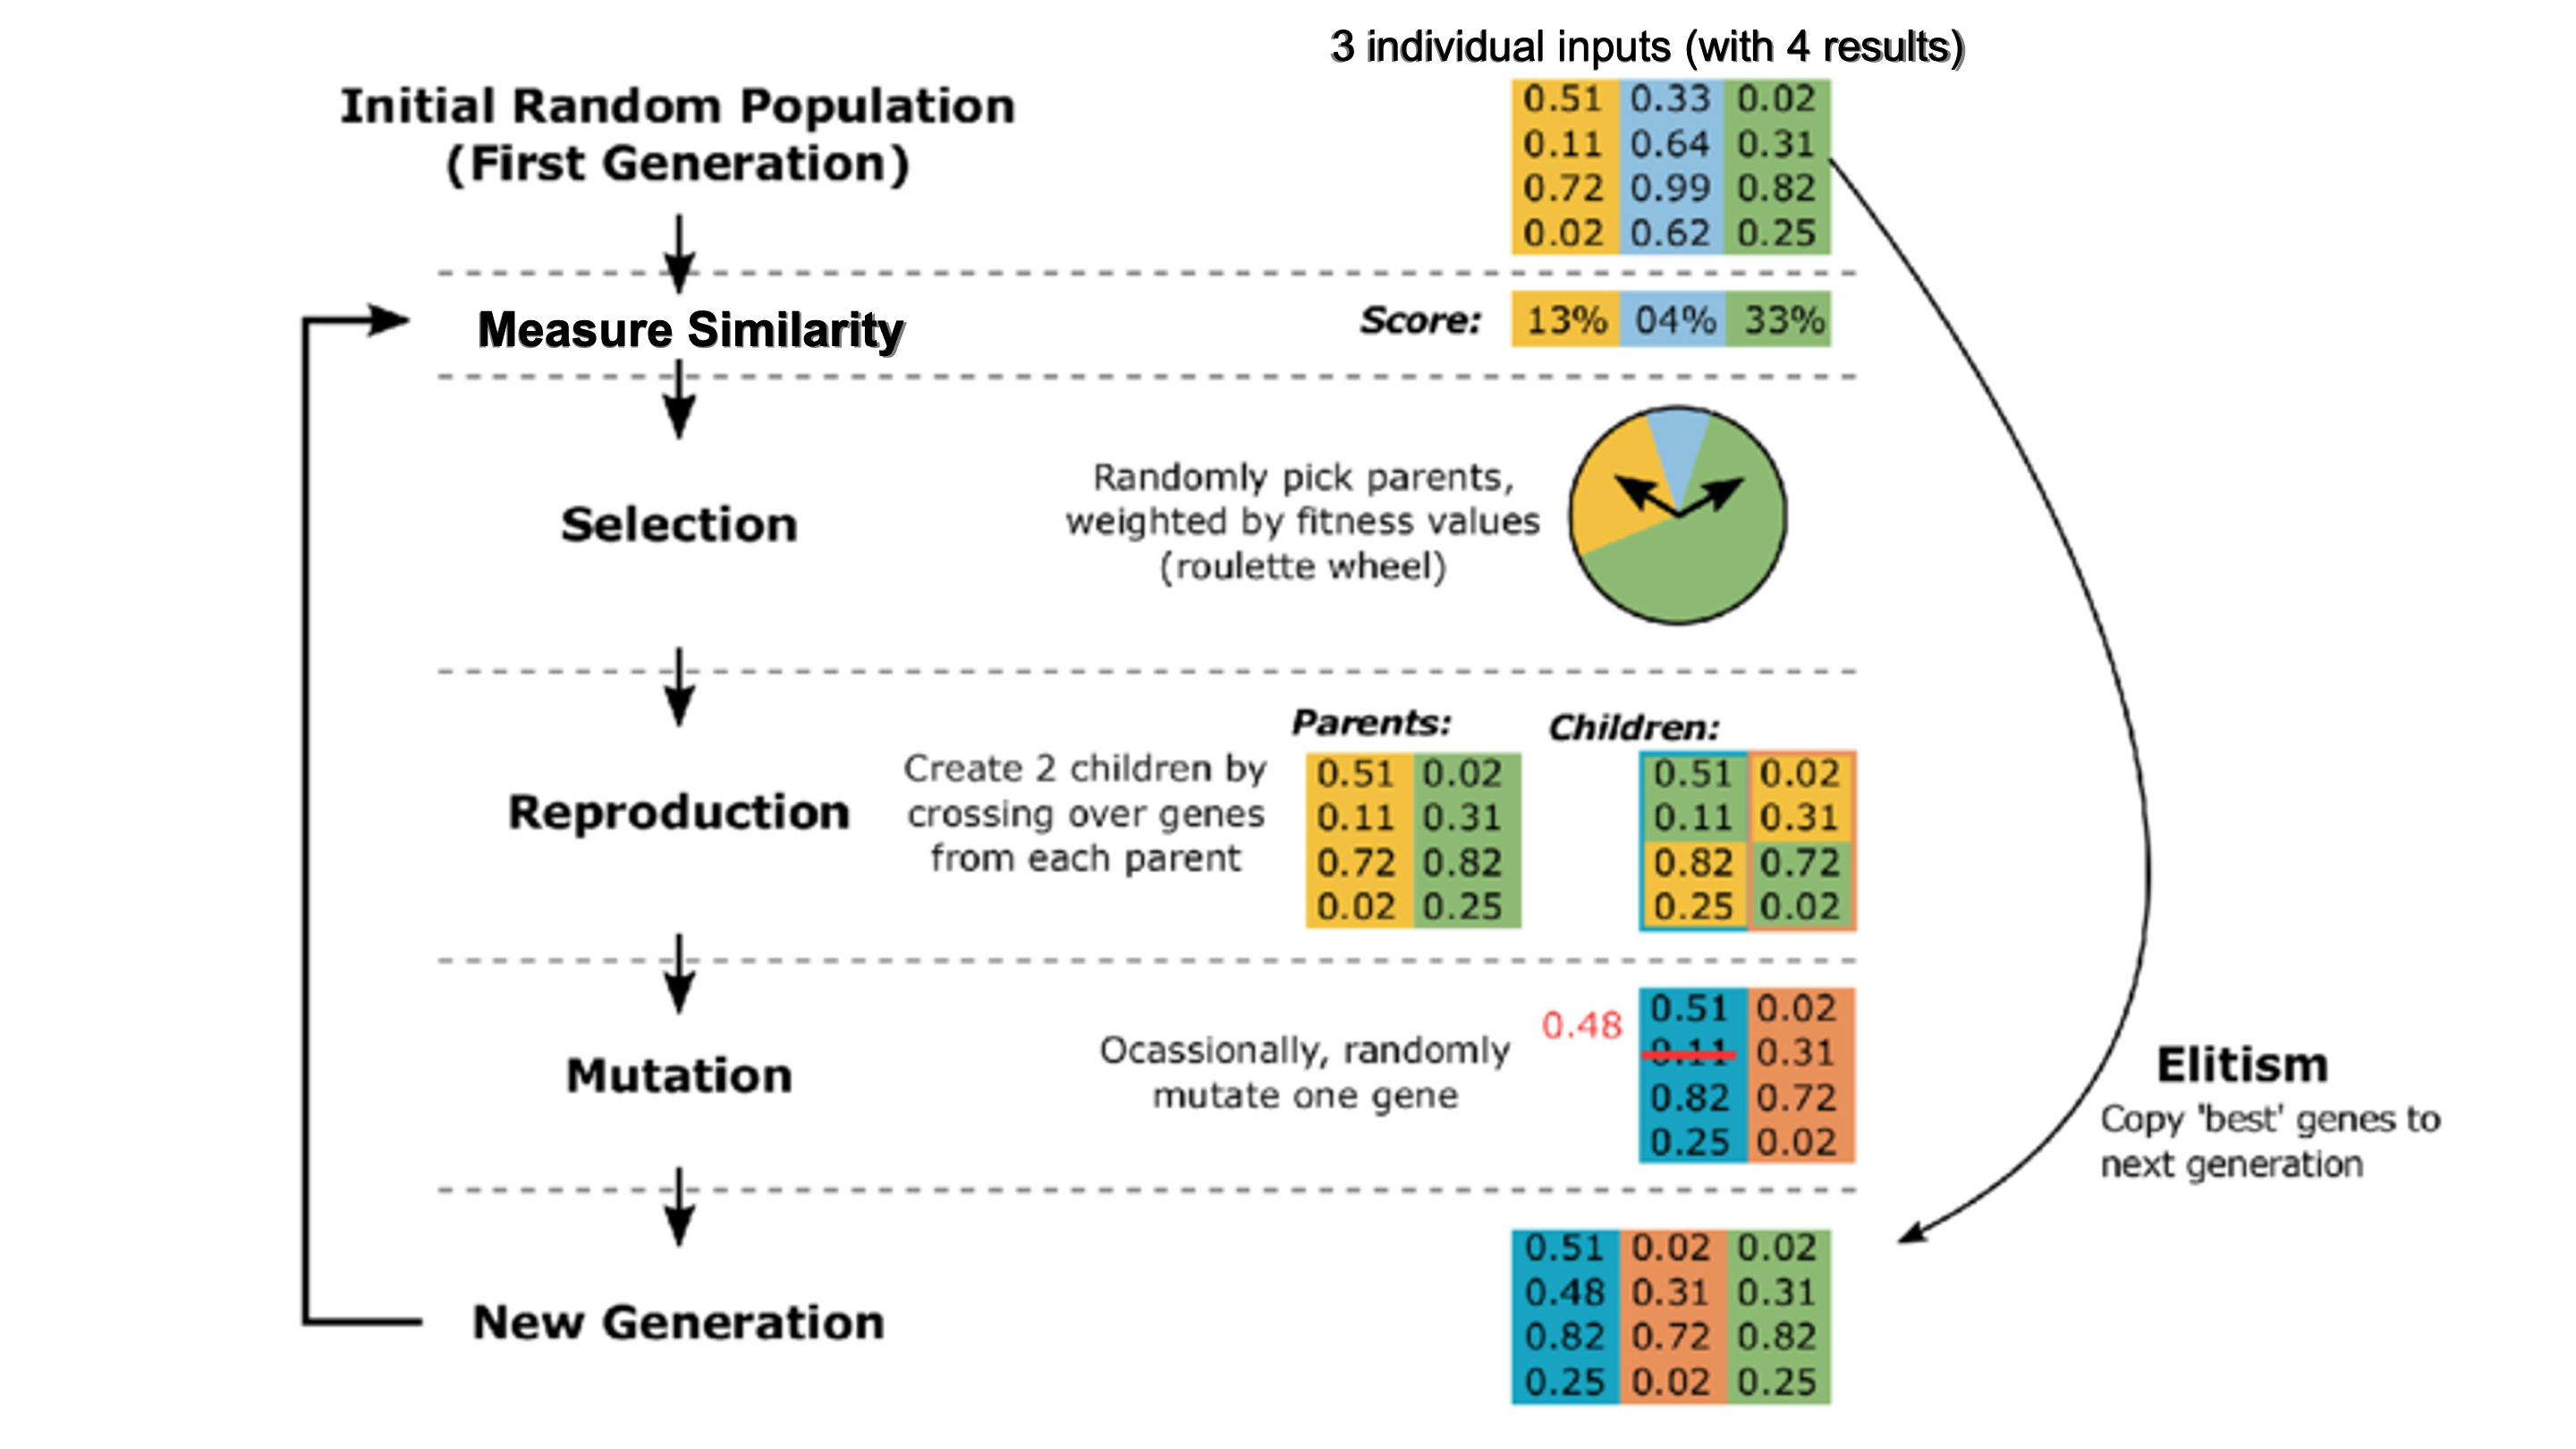
\includegraphics[width=1\textwidth]{images/GA_concept.png}
	\caption{Genetic Algorithm Concept \protect}
	\label{fig:Genetic Algorithm Concept}
\end{figure}

\end{comment}

Results will be captured in three independent groupers: Named APT Groups, Country based Groups, and the combination of Country Separated Groups and Malware Family Groups.  Named APT Groups is the broadest group because it includes indirect state-sponsored threat actors, like intermediate level threat actors aimed at financial and educational institutions.  Country Separated Groups are further restricted to state-sponsored threat actors that are directly attributable to a country and commonly attack infrastructure based on a military, economic, or geopolitical goals.  The Country Separated Malware Family Groups further restricts classification down to the differences between the indirectly and directly sponsored, along with the differences in unique identifiers based on samples obtained. 

The other guiding force to measure the results will be to calculate the cost of the genetic algorithms' assistance in feature selection within the 13 different date types to be compared.  These features and the frequency of the data contained within this dataset are detailed in Figure 3.3, titled Features.  With the cost results captured, statistical analysis on the dissimilar features included in this correlation will be scaled to larger datasets in order to find a use-able balance between expert selection and genetic algorithm feature enumeration of dissimilar results.  

The hypothesis will be validated using the correlation-based ESGA method for feature selection algorithm described in the feature pruning section.  This research will be validated by measuring the accuracy of attribution within the chosen feature sets.  The environment for this research will be a combination of three main items: a dataset of attributed malware, an automated analytical platform, and algorithms for classification.  The dataset includes 3594 samples from 12 different APTs. \cite{APTMalware2022}  These samples were chosen because they are from different APTs supporting different countries and contain a variety of unique information that can be used to test the efficiency of applying cyber threat attribution.  Details on the samples and traceability to cyber threat intelligence report applying attribution is contained within the overview.csv file within the root directory of the dataset.  The automated analytical platform is a malware sandbox and software codebase to manage actions.  Examples of actions managed by the codebase is interactions with the sandbox api to submit and collect samples, pruning of results, execution of NLP, and reporting of results.

The timeline for research defense, code changes, data collection, analysis, and reporting on this research is planned for in the following timeline.
% Create unordered list in LaTeX
\begin{itemize}
  \item Defend Research Proposal, April 2023
  \item Implement Code Changes for Research, May 2023
  \item Collect and Verify Data, June 2023
  \item Document Results, July 2023
  \item Defend Research, August, 2022
\end{itemize}

\begin{comment}
\begin{table}[]
\begin{tabular}{lll}
Format   & Provider       & URL                                                                  \\
misp     & CIRCL          & https://www.circl.lu/doc/misp/feed-osint                             \\
misp     & Botvrij.eu     & https://www.botvrij.eu/data/feed-osint                               \\
freetext & cinsscore.com  & https://cinsscore.com/list/ci-badguys.txt                            \\
csv      & cybercure.ai   & https://api.cybercure.ai/feed/get\_ips?type=csv                      \\
csv      & cybercure.ai   & https://api.cybercure.ai/feed/get\_url?type=csv                      \\
freetext & IPsum          & https://raw.github.com/stamparm/ipsum/master/levels/2.txt \\
freetext & spamhaus.org   & https://www.spamhaus.org/drop/drop.txt                               \\
freetext & sans.edu       & https://isc.sans.edu/block.txt                                       \\
freetext & multiproxy.org & http://multiproxy.org/txt\_all/proxy.txt                             \\
freetext & multiproxy.org & http://multiproxy.org/txt\_anon/proxy.txt                            \\
freetext & torproject.org & https://check.torproject.org/exit-addresses                          \\
freetext & rutgers.edu    & https://report.cs.rutgers.edu/DROP/attackers                         \\
freetext & sans.edu       & https://isc.sans.edu/feeds/topips.txt                               
\end{tabular}
\end{table}

\begin{figure}
	\centering
	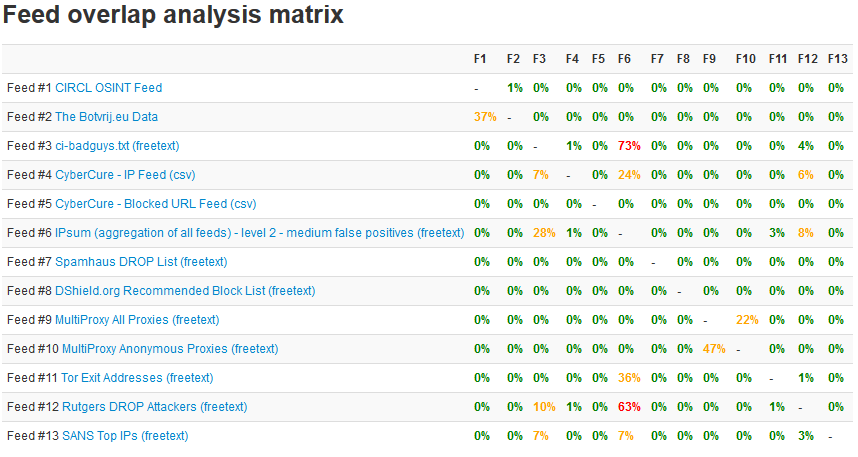
\includegraphics[width=1\textwidth]{images/MISP_FeedOverlap.PNG}
	\caption{MISP Feed Overlap}
	\label{fig:MISP Feed Overlap}
\end{figure}

The novel framework described earlier in the paper based upon a tiered foundation will be used to apply analysis to like inputs.  The Cyber Kill Chain will be used to describe a threats actions in terms of a foundation based on the stages of reconnaissance, exploitation, and effects.  The MITRE ATT\&CK framework will be used to describe specific action within the stage of exploitation.  Vulnerability details will be applied form input from the NVD.

From this framework, training data will be exported to a augmented intelligence platform designed for NLP and training will take place to enable authorship attribution.



\subsection{Validation Outline}

\begin{outline}[enumerate]
\let\OldOne\1%
\let\OldTwo\2%
\let\OldThree\3%
\renewcommand*{\1}{\normalsize\normalfont\OldOne\bfseries\Large\scshape}%
\renewcommand*{\2}{\normalsize\normalfont\OldTwo\bfseries}%
\renewcommand*{\3}{\normalsize\normalfont\OldThree\small}%
\1 Setup system to analyze malware in datasets A and B
    \2 Collect software's attributes from dataset A, then B
        \3 syntax, functions, inputs, outputs, return values, comments, etc
    \2 Apply 3 level framework
        \3 Cyber Kill Chain (foundation - recon, exploitation, effect)
        \3 MITRE ATTACK (exploitation)
        \3 NVD (effect)
    \2 Apply Cyber Threat Attribution
\1 setup system to compare results 
\end{outline}


DU commnet on 'malicous software samples' =
		"specifics needed: where will they come from (if known)?"
		"how many samples will you need?"
		"type of samples... binaries, or?"

	DU comment "Tensorflow and PyTorch are implementations.  What are the types of ML algorithums you plan to employ?"

	DU comment on 'either confirm or disagree with' = "How are you going to confim/disagree?  Statistical details?"

	validation - prove out the hypothosis is missing
		validation plan - how are we going to measure it (show that the null hyposotis is disproved)

	DU "Schedule of milestones would be much appriciated"

	Milestone Schedule - Months of work to take placee

Notes:
passive voice is a small no-no, use active voice
\end{comment}

\begin{comment}
The research hypothesis will be validated by exploring two approaches to implementing experimental software correlation mapping.  The first entails building and identifying models from malicious software samples using the TensorFlow open source software library for numerical computation using data flow graphs in order to map capabilities and trends.  \cite{kolosnjaji2016deep}  The second building and identifying models from malicious software samples by using the Pytorch open source software library for processing variable length inputs and outputs in order to map capabilities and trends.  \cite{pytorch:2017}

The first method is to implement software correlation mapping could be to emulate mathematical models using TensorFlow in order to apply known semantic characteristics against malicious software samples.  This could be the implementation of a black box technique for adversarial authorship.  The software correlation mapping could be created using the linguistic unit chains created by the authors as part of the identification and trend analysis.  Research into the vector representation of words using TensorFlow has been shown to have a computationally efficient model for learning word embeddings in natural language processing systems.  \cite{mikolov2013efficient}

The second method will be implement by processing variable length inputs and outputs from the malicous samples in order to highlight and them execute trend analysis against the semantic characteristics.  A framework build for binary and static code analysis could be used to create semantically correct representations of capabilities and potentiality motivations with this representation.

For the validation suite of this research a description of what properties that can be used to either confirm or disagree with the research findings are below.  These properties include the application of natural language processing to combine phrases, comments, statements, functions, build details, and other pieces of data in order to understand author's self-interpreted decision trees and apply them to like samples.  For this research the validation suite consists of a scalable testing infrastructure and various families of test cases for common software languages that malicious software is created in.  The test cases aim to identify and resolve differences and similarities within software for which relationships can be applied.  The framework of this test suite is intended to be robust enough to scale up to test cases for the future releases of increasing complexity.  This validation suite, along with review of the relevant literature, aim to ensure the results are reasonable.

These methods will be tested by applying open-source projects on a sample of hardware platforms, to be determined later, where source and compiled code can be obtained to verify semantic changes as well as to allow for refactoring of the mapping process in order to test all these differencing techniques' ability to apply attribution and gauge future capabilities.



\section{Schedule}
% http://texdoc.net/texmf-dist/doc/latex/pgfgantt/pgfgantt.pdf

Below is the schedule for research and validation in the form of a gantt chart.

% \definecolor{barblue}{RGB}{153,204,254}
\definecolor{barblue}{RGB}{246,119,34}
% \definecolor{groupblue}{RGB}{51,102,254}
\definecolor{groupblue}{RGB}{73,110,156}
\definecolor{linkred}{RGB}{165,0,33}
\renewcommand\sfdefault{phv}
\renewcommand\mddefault{mc}
\renewcommand\bfdefault{bc}
\setganttlinklabel{s-s}{START-TO-START}
\setganttlinklabel{f-s}{FINISH-TO-START}
\setganttlinklabel{f-f}{FINISH-TO-FINISH}
\sffamily
\begin{ganttchart}[
    canvas/.append style={fill=none, draw=black!5, line width=.75pt},
    hgrid style/.style={draw=black!5, line width=.75pt},
    vgrid={*1{draw=black!5, line width=.75pt}},
    today=0,
    today rule/.style={
        draw=black!64,
        dash pattern=on 3.5pt off 4.5pt,
        line width=1.5pt
    },
    today label font=\small\bfseries,
    title/.style={draw=none, fill=none},
    title label font=\bfseries\footnotesize,
    title label node/.append style={below=7pt},
    include title in canvas=false,
    bar label font=\mdseries\small\color{black!70},
    bar label node/.append style={left=2cm},
    bar/.append style={draw=none, fill=black!63},
    bar incomplete/.append style={fill=barblue},
    bar progress label font=\mdseries\footnotesize\color{black!70},
    group incomplete/.append style={fill=groupblue},
    group left shift=0,
    group right shift=0,
    group height=.5,
    group peaks tip position=0,
    group label node/.append style={left=.6cm},
    group progress label font=\bfseries\small,
    link/.style={-latex, line width=1.5pt, linkred},
    link label font=\scriptsize\bfseries,
    link label node/.append style={below left=-2pt and 0pt}
    ]{1}{16}
\gantttitle[
    title label node/.append style={below left=7pt and -3pt}
]{WEEKS:\quad1}{1}
\gantttitlelist{2,...,16}{1} \\
\ganttgroup[progress=0]{1. Written Defense of Research}{1}{16} \\
\ganttbar[
    progress=0,
    name=WBS1A
]{\textbf{1.1} Dataset analysis}{1}{6} \\
\ganttbar[
    progress=0,
    name=WBS1B
]{\textbf{1.2} Apply Framework}{7}{12} \\
\ganttbar[
    progress=0,
    name=WBS1C
]{\textbf{1.3} Apply Attribution}{7}{12} \\
\ganttbar[
    progress=0,
    name=WBS1D
]{\textbf{1.4} Compare Results}{13}{16}
\ganttlink[link type=f-s]{WBS1A}{WBS1B}
\ganttlink[link type=s-s]{WBS1B}{WBS1C}
\ganttlink[link type=f-s]{WBS1C}{WBS1D}
\end{ganttchart}
\end{comment}

%**************************************************************************
%**************************************************************************
%FIN
%**************************************************************************
%**************************************************************************

\bibliographystyle{ACM-Reference-Format-Journals}
\bibliography{Remote}
\end{document}
